
\newpage

\section{ACEF to Siconos}
\subsection{The MLCS formulation}
\subsubsection{The MLCS from the automatic formulation}
 \begin{eqnarray}
A_{x'}x'=A_{x}x +A_{z}Z_{s} +A_{\lambda} \lambda +a(t)&\label{eq2}\\
0=B_{x}x+B_{z}Z_{s} + B_{\lambda}\lambda + b(t)&\label{eq3}\\
Y=C_{x}x+C_{z}Z_{s}+C_{\lambda}\lambda + c(t) &\label{eq4}\\
0 \leq Y \, \perp \, \lambda \geq 0&\label{eqperp}
\end{eqnarray}
 With $A_{x'}$ regular.\\
 Let
 \begin{itemize}
  \item[--] Let n the x dimension.
  \item[--] Let m the Y dimension.
  \item[--] Let s the $Z_{s}$ dimension.
\end{itemize}

\subsubsection{Rappel, siconos model}
Siconos allow to define some dynamical systems with some relations:
\[Mx'=Ax +b(t)+R\]
\[Y=CX +D \lambda\]
\[r=B \lambda\]
\subsubsection{concataining $Z_{s}$ and $\lambda$ }
To fit the acef formulation in the siconos model, a first way could be to concataining the vectors $Z_{s}$ and $\lambda$, it rises to the following system:
 \begin{eqnarray}
Mx'=Ax +B_{1} \lambda +a(t)&\label{eq_merge_1}\\
0=B_{x}x+ B_{2}\lambda + b(t)&\label{eq_merge_2}\\
Y=Cx+D\lambda + c(t) &\label{eq_merge_3}\\
(\lambda_{1},..,\lambda_{s}) free\\
0 \leq Y \, \perp \, (\lambda_{s+1},..,\lambda_{s+m})^{t} \geq 0&\label{eq_merge_eqperp}
\end{eqnarray}

There are tow disadvantages with this formulation:
\begin{itemize}
 \item[--] The time discretisation of the Zs variables like the complementarity variables is not
enough accuracy.
 \item[--] Because of the equality, it is not compatible with the block siconos structure.
\end{itemize}
\subsubsection{concataining x and $Z_{s}$ }
An other solution could be to concataining the vector x and $Z_{s}$, it leads to the following
system:
 \begin{eqnarray}
Mx'=Ax +B \lambda +a(t)&\label{eq_merge2_1}\\
Y=Cx+D\lambda + c(t) &\label{eq_merge2_3}\\
0 \leq Y \, \perp \, \lambda \geq 0&\label{eq_merge2_eqperp}
\end{eqnarray}
In this case, M is not regular, it is a DAE. The main objection is that the semi-explicit form of
the DAE is hidden. But the physical variables are all discretised with the same model, moreover it
is compatible with the block structure of siconos.

\subsection{Example, one DS and n UR}

This section describe the case of a system with one DS, and n UR from the same interaction. The n UR
comes from n NS components defined by the same geometry :

\begin{equation}\left(\begin{array}{c}
\beta = Z_{nsi} = A_{i}x+B\lambda_{i} + a_{i}\\
y_{i}=D_{i}x+F\lambda_{i}+e_{i}\\
0 \leq y_{i} \, \perp \, \lambda_{i} \geq 0
\end{array}\right)
\end{equation}
where $Z_{nsi}$ is some physical variables. In siconos, it is contained in the Non Smooth Law of the
interaction.

\begin{equation}\left(\begin{array}{c}
Mx = Ax + B \lambda\\
Y=(y_{1},...,y{n})^{t}=Cx + \left(\begin{array}{ccc} F & .. & 0\\ ..& F & ..\\0 & .. &
F\end{array}\right) \lambda\\
ie \qquad Y=Cx+D\lambda\\
0 \leq Y \, \perp \, \lambda \geq 0
\end{array}\right)
\end{equation}



\subsubsection{A MLCP formulation in Siconos}
The Dynamic system:
\[Mx'=Ax +B \lambda +b(t)\]
\[y=Cx +D \lambda +e(t)\]
Discretisation:
\[M(x(t_{i+1})-x(t_{i}))=h(\theta A x(t_{i+1}) + (1-\theta) A x(t_{i}) +B \lambda (t_{i+1}) +\theta
b(t_{i+1}) + (1-\theta) b(t_{i}))\]
\[Wx(t_{i+1})=hB \lambda (t_{i+1}) + f_{free}\]
with:
\[f_{free}=h(1-\theta) A x(t_{i}) + Mx(t_{i})+h \theta b(t_{i+1}) + h(1-\theta) b(t_{i}) \qquad W=(M-h\theta A)\]
\[y(t_{t+1})=Cx(t_{i+1}) +D \lambda(t_{i+1}) +e(t_{i+1})\]
MLCP instance:
\[w=Mz+q\]
\[w=\left(\begin{array}{c}0\\y(t_{i+1})\end{array}\right) \qquad
z=\left(\begin{array}{c}x(t_{i+1})\\ \lambda (t_{i+1})\end{array}\right)\]
\[q=\left(\begin{array}{c}f_{free}\\ e(t_{i+1})\end{array}\right)\]
\[M=\left(\begin{array}{cc}-W&hB\\ C&D\end{array}\right)\]
\newpage
\subsection{Simulation DAE/ODE comparaison}
The following graphic compares the diodes bridges simulations from the DAE and the ODE model. Because of the time
discretisation, the DAE simulation is less damping.
\begin{figure}[h]
%GNUPLOT: LaTeX picture with Postscript
\begin{picture}(0,0)%
\includegraphics{DAE_ODE.eps}%
\end{picture}%
\begingroup
\setlength{\unitlength}{0.0200bp}%
\begin{picture}(18000,10800)(0,0)%
\put(1925,1650){\makebox(0,0)[r]{\strut{} 0}}%
\put(1925,2510){\makebox(0,0)[r]{\strut{} 1}}%
\put(1925,3370){\makebox(0,0)[r]{\strut{} 2}}%
\put(1925,4230){\makebox(0,0)[r]{\strut{} 3}}%
\put(1925,5090){\makebox(0,0)[r]{\strut{} 4}}%
\put(1925,5950){\makebox(0,0)[r]{\strut{} 5}}%
\put(1925,6810){\makebox(0,0)[r]{\strut{} 6}}%
\put(1925,7670){\makebox(0,0)[r]{\strut{} 7}}%
\put(1925,8530){\makebox(0,0)[r]{\strut{} 8}}%
\put(1925,9390){\makebox(0,0)[r]{\strut{} 9}}%
\put(1925,10250){\makebox(0,0)[r]{\strut{} 10}}%
\put(2200,1100){\makebox(0,0){\strut{} 0}}%
\put(3698,1100){\makebox(0,0){\strut{} 0.0005}}%
\put(5195,1100){\makebox(0,0){\strut{} 0.001}}%
\put(6693,1100){\makebox(0,0){\strut{} 0.0015}}%
\put(8190,1100){\makebox(0,0){\strut{} 0.002}}%
\put(9688,1100){\makebox(0,0){\strut{} 0.0025}}%
\put(11185,1100){\makebox(0,0){\strut{} 0.003}}%
\put(12683,1100){\makebox(0,0){\strut{} 0.0035}}%
\put(14180,1100){\makebox(0,0){\strut{} 0.004}}%
\put(15678,1100){\makebox(0,0){\strut{} 0.0045}}%
\put(17175,1100){\makebox(0,0){\strut{} 0.005}}%
\put(550,5950){\rotatebox{90}{\makebox(0,0){\strut{}R voltage}}}%
\put(9687,275){\makebox(0,0){\strut{}time (s)}}%
\put(14950,9675){\makebox(0,0)[r]{\strut{}ODE}}%
\put(14950,9125){\makebox(0,0)[r]{\strut{}DAE}}%
\end{picture}%
\endgroup
\endinput

\end{figure}
\newpage
\subsubsection{Building a NonSmooth Dynamical System}
 
 aDS = new FirstOrderLinearDS$(int,A_{x'},A_{x},a(t))$;\\
 aTIR = new FirstOrderLinearTIR$(\left(\begin{array}{c}B_{x}\\C_{x}
 \end{array}\right),0,\left(\begin{array}{c}B_{\lambda}\\C_{\lambda}
 \end{array}\right),\left(\begin{array}{c}b(t)\\c(t) \end{array}\right),A_{\lambda})$\\

 aNSL= new complementarityConditionNSL(m);\\
 aI = new interaction(``MLCP'',allDS,1,m+s, aNSL, aTIR);\\
 aNSDS= new NonSmoothDynamicalSystem(aDS, aI);\\
 aM=new Model($t_{0}$,T);\\
 aM setNSDS(aNSDS);\\
\\
\subsubsection{Simulation}
aTD = new TimeDiscretisation(h,aM);\\
aS = new TimeStepping(aTD);\\
aMoreau = new Moreau(aDS,0.5,aS);\\
aMLCP = new MLCP(aM,mySolver,''MLCP'');\\
aS init();\\
aS run();\\
\newpage

\section{Initial conditions}
\subsection{Initial conditions in NGSPICE}
In spice, the initial conditions are about the Voltage node. It is not possible to specify a
current. The DC analysis consists in computing the operating point of the circuit with inductors
shorted and capacitor opened. There are three ways to define the initial conditions(description from NGSPICE User Manual):

\subsubsection{.NODESET: Specify initial node voltage guesses}
It consists in doing a DC analysis. The initial node voltage are used to initialize the DC analysis,
but the iteration continues to the true solution.
\subsubsection{.IC: set initial condition }
It consists in doing a DC analysis. But the specify node voltage values are forced during the DC
iterations. It is the preferred method since it allows NGSPICE to compute a consistent DC solution.
\subsubsection{.IC and UIC: set initial condition }
In this case there are no DC analysis. The specified values are directly used for the trans
analysis.

\subsection{Initial conditions in ACEF}
In current version r84.\\
\subsubsection{.IC interpretation}
In ACEF there are no DC analysis. The initial node voltage values are used to initialize the
dynamical unknowns of type TENSION.
\subsubsection{It could be better to do}
First point, note that inductors shorted and capacitor opened means $\frac{dx}{dt}=0$. Because:\\
The capacitor constitutive law is : $C\frac{dU}{dt}=I$. If the capacitor branch is opened, it means
$I=0$. So $C\frac{dU}{dt}=0$.\\
The inductor constitutive law is : $L\frac{dI}{dt}=U$. If the inductor branch is shorted, it means
$U=0$. So $C\frac{dI}{dt}=0$.\\
Second point, all the node potential are unknowns included in the $Z_{s}$ vector with ACEF, or in
$\lambda$ vector with current version of SICONOS.\\

It leads to the following system:

 \begin{eqnarray}
0=A_{x}x_{0} +A_{\lambda} \lambda +a(t)\\
0=B_{x}x_{0}+ B_{\lambda}\lambda + b(t)\\
Y_{0}=C_{x}x_{0}+C_{\lambda}\lambda + c(t) \\
\lambda_{i} = \lambda_{i0} \qquad for \qquad i \in \{ user initial value \}\\
\lambda_{i} \qquad free \qquad i \notin \{ user initial value \}\\
0 \leq Y_0 \, \perp \, (\lambda_{s+1},..,\lambda_{s+m})^{t} \geq 0
\end{eqnarray}
The solution $x_{0}$ and $\lambda_{1}...\lambda_{s}$ are the initial values for the trans analysis.
\newpage

\section{MLCP solver direct}
The standard MLCP description:
\[n=dim(z_{1}) \qquad m=dim(z_{2})\]
\[M \left(\begin{array}{c} z_{1}\\z_{2} \end{array}\right)+\left(\begin{array}{c} a\\b \end{array}\right)=\left(\begin{array}{c} 0\\w_{2}\\ \end{array}\right)\]
\[0 \leq z_{2} \, \perp \, w_{2} \geq 0\]
\[M=\left(\begin{array}{cc} A&C\\B&D \end{array}\right)\]
The direct solver consists in solving a MLCP when complementarity condition is known. It leads to a
linear system.
\[I_{z} \cup I_{w} = \{ 1,..,m\}\]
\[z_{2_{i}}=0 \qquad and \qquad w_{2_{i}} \geq 0 \qquad i \in I_{w} \]
\[w_{2_{i}}=0 \qquad and \qquad z_{2_{i}} \geq 0 \qquad i \in I_{z} \]

\subsection{First linear system formulation}
The MLCP becomes:\\
\[\label{system1} M_{1} \left(\begin{array}{c} z_{1}\\zw \end{array}\right)+\left(\begin{array}{c} a\\b
\end{array}\right)=0 \]
\[zw_{i}=w_{i} \qquad if \qquad i \in I_{w}\]
\[zw_{i}=z_{i} \qquad if \qquad i \in I_{z}\]
With $M_{1}$:
\[M_{1}=\left(\begin{array}{cc} A&E\\D&F \end{array}\right)\]
for $i \in I_w$:
\[E_{i}=C_{i} \qquad F_{i}=B_{i} \]
for $i \in I_z$:
\[E_{i}=0 \]
\[F_{i}=-e_{mi}\]
with $e_{mi}$ the $i^{th}$ vector base of $\RR^m$\\
The linear system \ref{system1} is solved, and the sign of the solution must be check.
\subsection{First linear system formulation}
The MLCP becomes:\\
\[\label{system2} M_{2} \left(\begin{array}{c} z_{1}\\ \widetilde{z_{2}}
\end{array}\right)+\left(\begin{array}{c} a\\ \widetilde{b}\end{array}\right)=0 \]
where $\widetilde{z_{2}}$ are the non null $z_{2}$ coordinates.\\
With $M_{2}$:
\[M_{2}=\left(\begin{array}{cc} A&\widetilde{C}\\D&\widetilde{B} \end{array}\right)\]

\[\label{system3} M_{3} \left(\begin{array}{c} z_{1}\\ \widetilde{z_{2}}
\end{array}\right)+\left(\begin{array}{c} a\\ \widetilde{\widetilde{b}}\end{array}\right)=\widetilde{\widetilde{W_{2}}} \]
where $\widetilde{\widetilde{w_{2}}}$ are the non null $w_{2}$ coordinates.
\[M_{3}=\left(\begin{array}{cc} D&G \end{array}\right)\qquad G_{ij}=B_{ij} \qquad i \in I_{w} \qquad
j \in I_{z}\]

\section{ACE/SICONOS simulation}

\subsection{Diode bridge simulation with acef}
%GNUPLOT: LaTeX picture with Postscript
\begin{picture}(0,0)%
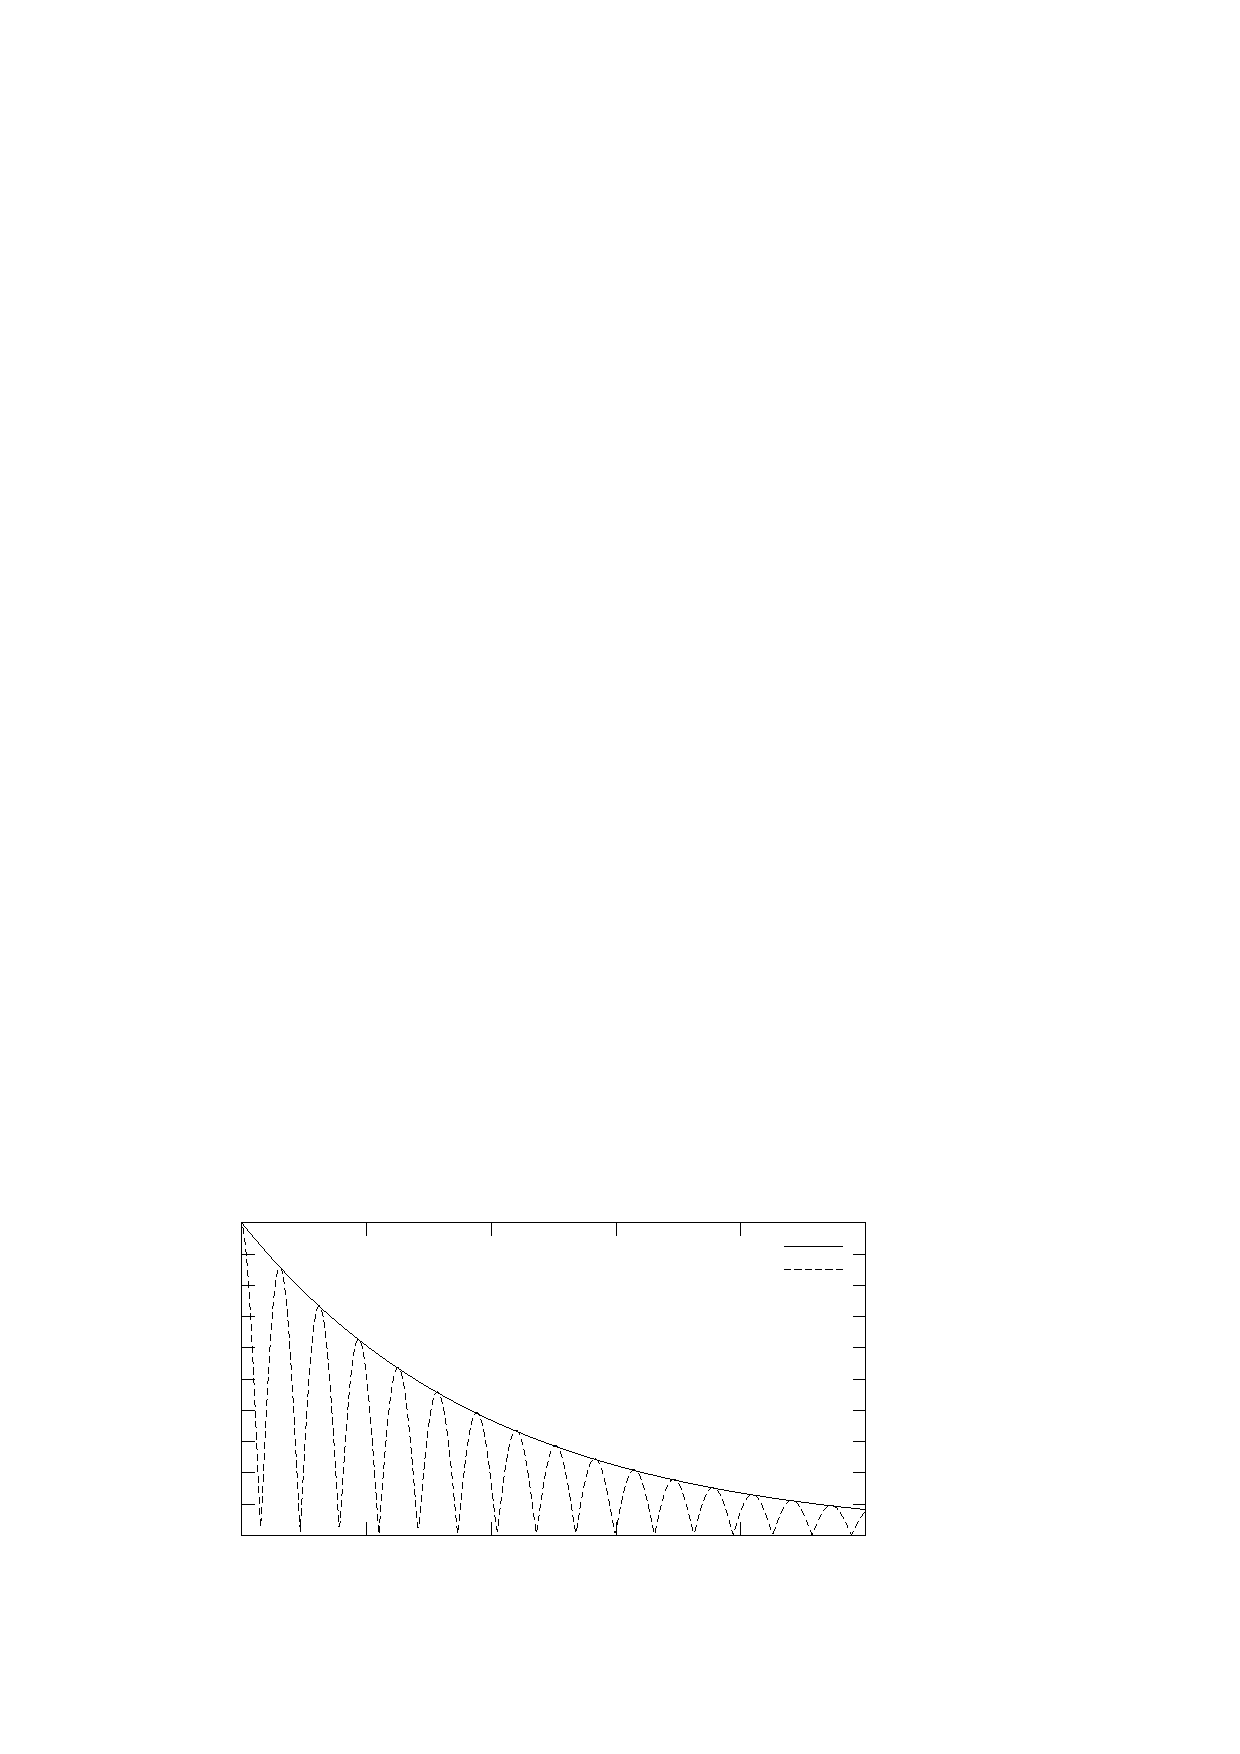
\includegraphics{DiodeBridgeAcef}%
\end{picture}%
\begingroup
\setlength{\unitlength}{0.0200bp}%
\begin{picture}(18000,10800)(0,0)%
\put(1925,1650){\makebox(0,0)[r]{\strut{} 0}}%
\put(1925,2400){\makebox(0,0)[r]{\strut{} 1}}%
\put(1925,3150){\makebox(0,0)[r]{\strut{} 2}}%
\put(1925,3900){\makebox(0,0)[r]{\strut{} 3}}%
\put(1925,4650){\makebox(0,0)[r]{\strut{} 4}}%
\put(1925,5400){\makebox(0,0)[r]{\strut{} 5}}%
\put(1925,6150){\makebox(0,0)[r]{\strut{} 6}}%
\put(1925,6900){\makebox(0,0)[r]{\strut{} 7}}%
\put(1925,7650){\makebox(0,0)[r]{\strut{} 8}}%
\put(1925,8400){\makebox(0,0)[r]{\strut{} 9}}%
\put(1925,9150){\makebox(0,0)[r]{\strut{} 10}}%
\put(2200,1100){\makebox(0,0){\strut{} 0}}%
\put(5195,1100){\makebox(0,0){\strut{} 0.001}}%
\put(8190,1100){\makebox(0,0){\strut{} 0.002}}%
\put(11185,1100){\makebox(0,0){\strut{} 0.003}}%
\put(14180,1100){\makebox(0,0){\strut{} 0.004}}%
\put(17175,1100){\makebox(0,0){\strut{} 0.005}}%
\put(550,5400){\rotatebox{90}{\makebox(0,0){\strut{}Ur}}}%
\put(9687,275){\makebox(0,0){\strut{}time}}%
\put(9687,9975){\makebox(0,0){\strut{}Diode bridge acef}}%
\put(14950,8575){\makebox(0,0)[r]{\strut{}10*exp(-x/(0.002))}}%
\put(14950,8025){\makebox(0,0)[r]{\strut{}"DiodeBridgeSimple.sim"}}%
\end{picture}%
\endgroup
\endinput

\\
This graphic validates the ACEF formulation, indeed the simulation follow the theoretical damping coefficient.
\subsection{Diode bridge simulation with siconos}
%GNUPLOT: LaTeX picture with Postscript
\begin{picture}(0,0)%
\includegraphics{DiodeBridgeSiconos.eps}%
\end{picture}%
\begingroup
\setlength{\unitlength}{0.0200bp}%
\begin{picture}(18000,10800)(0,0)%
\put(1925,1650){\makebox(0,0)[r]{\strut{} 0}}%
\put(1925,3150){\makebox(0,0)[r]{\strut{} 2}}%
\put(1925,4650){\makebox(0,0)[r]{\strut{} 4}}%
\put(1925,6150){\makebox(0,0)[r]{\strut{} 6}}%
\put(1925,7650){\makebox(0,0)[r]{\strut{} 8}}%
\put(1925,9150){\makebox(0,0)[r]{\strut{} 10}}%
\put(2200,1100){\makebox(0,0){\strut{} 0}}%
\put(5195,1100){\makebox(0,0){\strut{} 0.001}}%
\put(8190,1100){\makebox(0,0){\strut{} 0.002}}%
\put(11185,1100){\makebox(0,0){\strut{} 0.003}}%
\put(14180,1100){\makebox(0,0){\strut{} 0.004}}%
\put(17175,1100){\makebox(0,0){\strut{} 0.005}}%
\put(550,5400){\rotatebox{90}{\makebox(0,0){\strut{}Ur}}}%
\put(9687,275){\makebox(0,0){\strut{}time}}%
\put(9687,9975){\makebox(0,0){\strut{}Diode bridge siconos}}%
\put(14950,8575){\makebox(0,0)[r]{\strut{}10*exp(-x/(0.002))}}%
\put(14950,8025){\makebox(0,0)[r]{\strut{}"resSiconosDiodeSimple.dat"}}%
\end{picture}%
\endgroup
\endinput

\\
This graphic shows that the simulation from siconos is not correct. The theoretical damping
coefficient is not following.
\subsection{Buck simulation with acef}
%GNUPLOT: LaTeX picture with Postscript
\begin{picture}(0,0)%
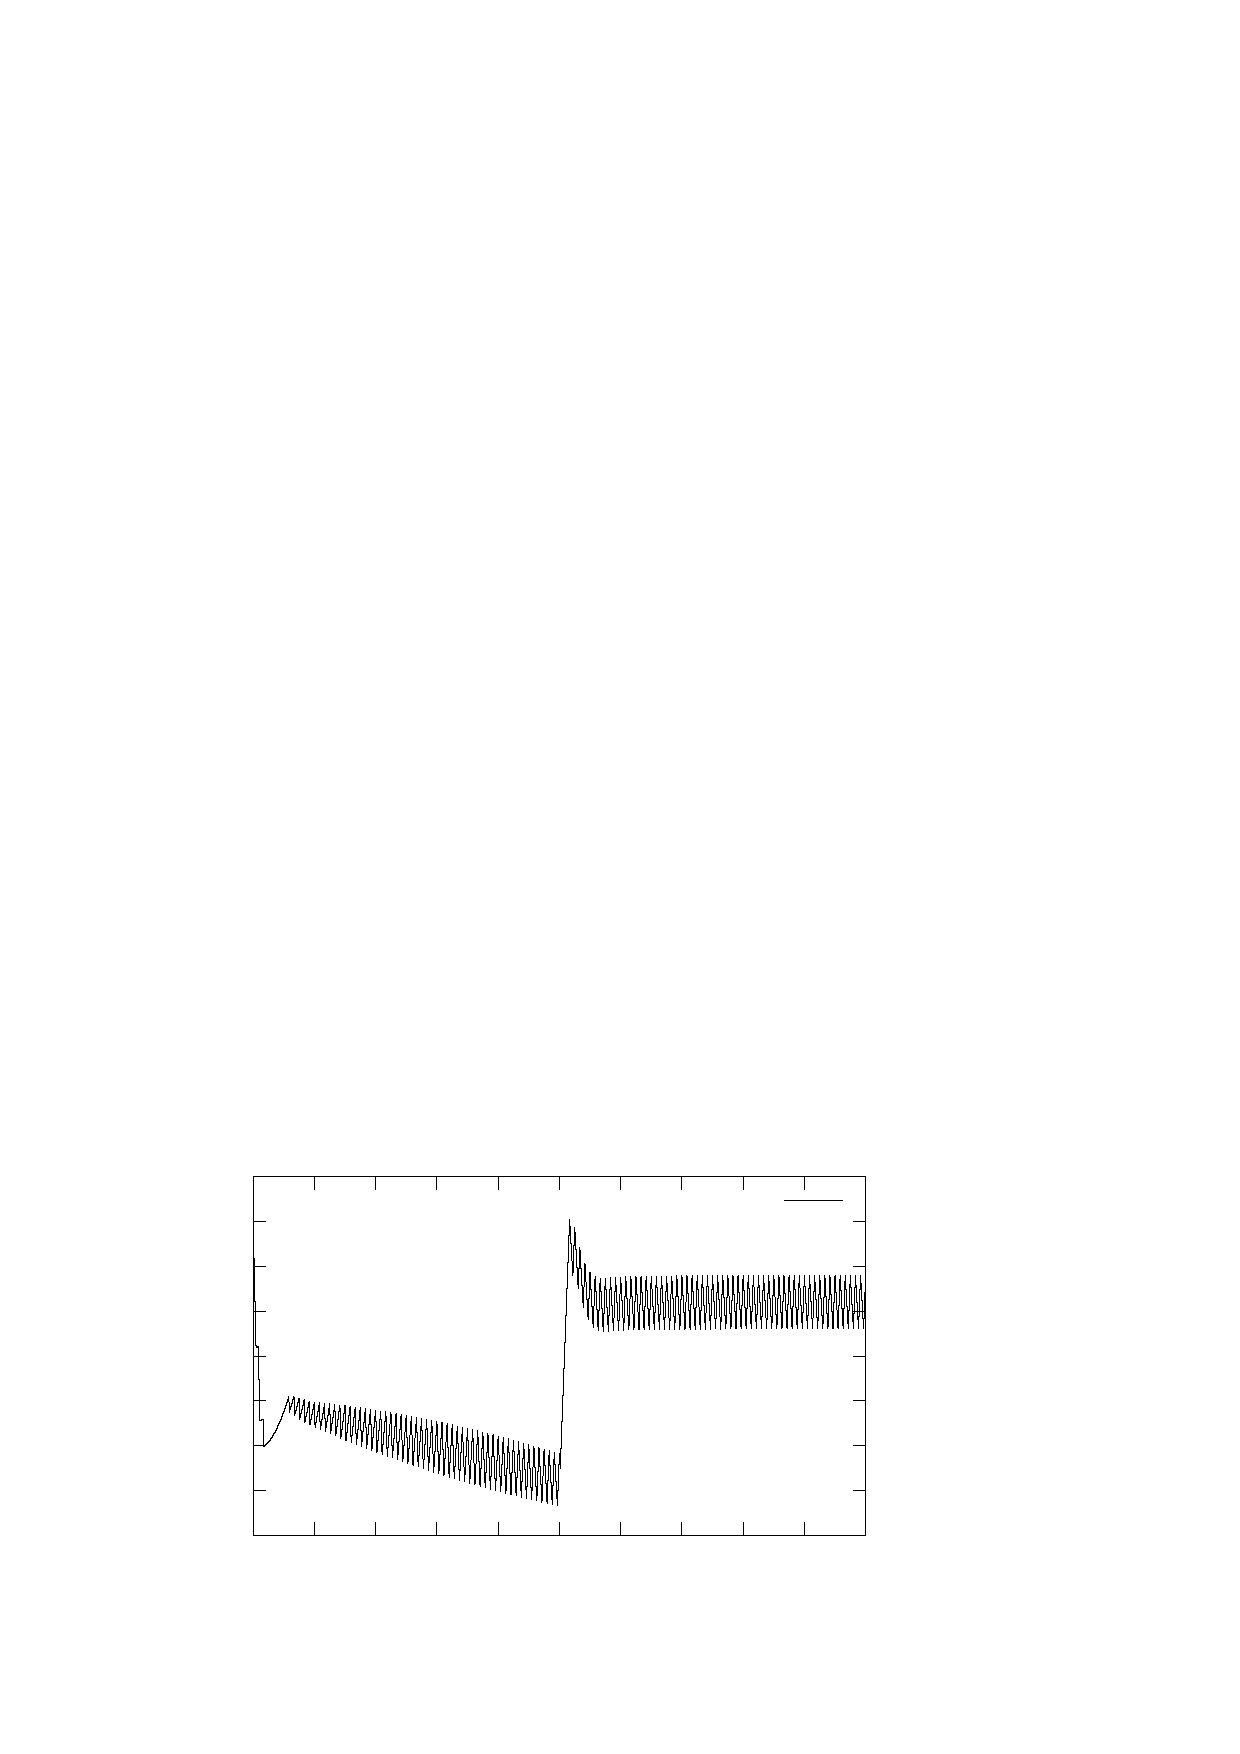
\includegraphics{Buck}%
\end{picture}%
\begingroup
\setlength{\unitlength}{0.0200bp}%
\begin{picture}(18000,10800)(0,0)%
\put(2200,1650){\makebox(0,0)[r]{\strut{}-0.7}}%
\put(2200,2725){\makebox(0,0)[r]{\strut{}-0.6}}%
\put(2200,3800){\makebox(0,0)[r]{\strut{}-0.5}}%
\put(2200,4875){\makebox(0,0)[r]{\strut{}-0.4}}%
\put(2200,5950){\makebox(0,0)[r]{\strut{}-0.3}}%
\put(2200,7025){\makebox(0,0)[r]{\strut{}-0.2}}%
\put(2200,8100){\makebox(0,0)[r]{\strut{}-0.1}}%
\put(2200,9175){\makebox(0,0)[r]{\strut{} 0}}%
\put(2200,10250){\makebox(0,0)[r]{\strut{} 0.1}}%
\put(2475,1100){\makebox(0,0){\strut{}   0}}%
\put(3945,1100){\makebox(0,0){\strut{}   2e-5}}%
\put(5415,1100){\makebox(0,0){\strut{}   4e-5}}%
\put(6885,1100){\makebox(0,0){\strut{}   6e-5}}%
\put(8355,1100){\makebox(0,0){\strut{}   8e-5}}%
\put(9825,1100){\makebox(0,0){\strut{}   1e-4}}%
\put(11295,1100){\makebox(0,0){\strut{}   1.2e-4}}%
\put(12765,1100){\makebox(0,0){\strut{}   1.4e-4}}%
\put(14235,1100){\makebox(0,0){\strut{}   1.6e-4}}%
\put(15705,1100){\makebox(0,0){\strut{}   1.8e-4}}%
\put(17175,1100){\makebox(0,0){\strut{}   2e-4}}%
\put(550,5950){\rotatebox{90}{\makebox(0,0){\strut{}Inductor current}}}%
\put(9825,275){\makebox(0,0){\strut{}time s}}%
\end{picture}%
\endgroup
\endinput

\\
\subsection{Buck simulation with siconos}
\input{BuckSiconos.tex}
\\
It is the same simulation. The relative difference between the simulation is $10^{-4}$, may be because
the time stepping is very small.
\newpage
\subsection{a sample example}
Consider the following circuit:\\
\begin{figure}[h]
\centerline{
 \scalebox{1.0}{
    \input{RC_.pstex_t}
 }
}\end{figure}
\\
With:
\begin{itemize}
  \item[--] C=1mF
  \item[--] R=100 Ohms
  \item[--] $V_{0}$=10 V
\end{itemize}

The circuit equation is :
\[C\frac{dV}{dt}=-\frac{V}{R}\]
The analytic solution is:
\[V(t)=V(0)\exp(-\frac{t}{RC})\]
Application Numeric: $V(0.01)=9.048...$\\
Start the discretisation with :\\
\[\int_{0}^{h}{RC\frac{dV(t)}{dt}+V(t)}dt=0\]
The implicit discretisation leads to :\\
With an implicit method:
\[RC(V_{h}-V_{0})+hV_{1}h=0 \qquad V_{h}=\frac{RCV_{0}}{RC+h}\]
Application Numeric: $V_{h}=9.091...$\\
The $\theta=0.5$ method leads to :
\[RC(V_{h}-V_{0})+0.5*h(V_{h}+V_{0})=0 \qquad V_{h} = \frac{RC-0.5h}{RC+0.5h}V_{0}\]
Application Numeric: $V_{h}=9.048...$\\
\subsubsection{A short justification}
\[\int_{0}^{h}{f(x)}dx = F(h)-F(0)\]
With a first order Taylor serie:
\[F(h+r)=F(h)+F'(h)r+o(r) \qquad F(0)=F(h)-f(h)h+o(h)\]
The implicit method order is 1.\\
With a DL2 Taylor:
\[F(h+r)=F(h)+F'(h)r+\frac{F''(h)r^2}{2}+o(r^2)\]
\[F(0)=F(h)-hf(h)+\frac{f'(h)h^2}{2}+o(h^2) \]
\[F(0)=F(h)-hf(h)+ (\frac{f(h)-f(0)}{h}+o(1)) \frac{h^2}{2}+o(h^2)\]
\[F(h)-F(0)=0.5(hf(h)+hf(0))+o(h^2)\]
The order is 2. 

\subsection{conclusion}
In current siconos version,the node voltage are integrated with an implicit method, and a $\theta$
is more accuracy.


\section{ DAE or ODE ?}

\subsection{Circuit without non smooth component}
In this section section, the circuit is composed only with linear components, capacitor, inductor,
resistor, voltage source, etc. The equation formulation leads to the following system:
\[ \]
\[0 = Cx + Dz \]
 \begin{eqnarray}
Mx'=Ax + Bz&\label{eq_cir_wout_NS_1}\\
0=Cx+ Dz &\label{eq_cir_wout_NS_2}\\
\end{eqnarray}
The equation \ref{eq_cir_wout_NS_2} comes from the Kirchhoff current laws.\\

The index of this DAE is 0, 1 or 2.
\subsection{Circuit with non smooth component}

\newpage
\section{delta sigma}
toto
\begin{figure}[h]
%GNUPLOT: LaTeX picture with Postscript
\begin{picture}(0,0)%
\includegraphics{DeltaSigmaSim.eps}%
\end{picture}%
\begingroup
\setlength{\unitlength}{0.0200bp}%
\begin{picture}(18000,10800)(0,0)%
\put(1650,1650){\makebox(0,0)[r]{\strut{}-3}}%
\put(1650,2900){\makebox(0,0)[r]{\strut{}-2}}%
\put(1650,4150){\makebox(0,0)[r]{\strut{}-1}}%
\put(1650,5400){\makebox(0,0)[r]{\strut{} 0}}%
\put(1650,6650){\makebox(0,0)[r]{\strut{} 1}}%
\put(1650,7900){\makebox(0,0)[r]{\strut{} 2}}%
\put(1650,9150){\makebox(0,0)[r]{\strut{} 3}}%
\put(1925,1100){\makebox(0,0){\strut{} 0}}%
\put(3450,1100){\makebox(0,0){\strut{} 1}}%
\put(4975,1100){\makebox(0,0){\strut{} 2}}%
\put(6500,1100){\makebox(0,0){\strut{} 3}}%
\put(8025,1100){\makebox(0,0){\strut{} 4}}%
\put(9550,1100){\makebox(0,0){\strut{} 5}}%
\put(11075,1100){\makebox(0,0){\strut{} 6}}%
\put(12600,1100){\makebox(0,0){\strut{} 7}}%
\put(14125,1100){\makebox(0,0){\strut{} 8}}%
\put(15650,1100){\makebox(0,0){\strut{} 9}}%
\put(17175,1100){\makebox(0,0){\strut{} 10}}%
\put(550,5400){\rotatebox{90}{\makebox(0,0){\strut{}tension}}}%
\put(9550,275){\makebox(0,0){\strut{}time}}%
\put(14950,8575){\makebox(0,0)[r]{\strut{}Vq1}}%
\put(14950,8025){\makebox(0,0)[r]{\strut{}Vsp1sn1}}%
\end{picture}%
\endgroup
\endinput

\end{figure}


\newpage
consider the following circuit:
\begin{figure}[h!]
\centerline{
 \scalebox{0.6}{
    \input{deltaSigma.pstex_t}
 }
}\end{figure}

\newpage
\section{Global error evaluation with the Buck converter}
It consists in computing the experimental order of the simulation. Since the analytic solution is
unknown, the reference trajectory is a simulation with a very small time step.
\subsection{Evaluation}
In the aim of compute the order of ACEF and Eldo, the following simulations have been performed:\\
\begin{tabular}{|c|c|c|c|c|c|c|c|c|}
\hline
Time stepping & 10 ps & 20 ps & 40 ps & 80 ps & 160 ps & 320 ps & 640 ps & 1200 ps \\
\hline
ELDO Global error & 150 pA & 443 pA & 966 pA & 2.1 nA & 4.5 nA & 8.2 nA & 20 nA & 34 nA \\
\hline
ACEF Global error & 246 pA & 513 pA & 1026 pA & 2.2 nA & 4.7 nA & 9.2 nA & 21 nA & 40 nA \\
\hline
ELDO Log2(global error)& -32.6 & -31 & -30 & -28.8  & -27.7 & -26.8 & -25.6 & -24.8 \\
\hline
ACEF Log2(global error)& -31.9 & -30.8 & -29.8 & -28.7  & -27.7 & -26.7 & -25.5 & -24.5 \\
\hline
\end{tabular}\\
\\
The 5ps trajectory is the reference trajectory used to compute the global error of the other
simulations. \\The following graphic shows the log2(Global error) as a function of log2(time
step):\\
%GNUPLOT: LaTeX picture with Postscript
\begin{picture}(0,0)%
\includegraphics{BuckGlobalError.eps}%
\end{picture}%
\begingroup
\setlength{\unitlength}{0.0200bp}%
\begin{picture}(18000,10800)(0,0)%
\put(1925,1650){\makebox(0,0)[r]{\strut{}-33}}%
\put(1925,2483){\makebox(0,0)[r]{\strut{}-32}}%
\put(1925,3317){\makebox(0,0)[r]{\strut{}-31}}%
\put(1925,4150){\makebox(0,0)[r]{\strut{}-30}}%
\put(1925,4983){\makebox(0,0)[r]{\strut{}-29}}%
\put(1925,5817){\makebox(0,0)[r]{\strut{}-28}}%
\put(1925,6650){\makebox(0,0)[r]{\strut{}-27}}%
\put(1925,7483){\makebox(0,0)[r]{\strut{}-26}}%
\put(1925,8317){\makebox(0,0)[r]{\strut{}-25}}%
\put(1925,9150){\makebox(0,0)[r]{\strut{}-24}}%
\put(2200,1100){\makebox(0,0){\strut{} 3}}%
\put(4072,1100){\makebox(0,0){\strut{} 4}}%
\put(5944,1100){\makebox(0,0){\strut{} 5}}%
\put(7816,1100){\makebox(0,0){\strut{} 6}}%
\put(9688,1100){\makebox(0,0){\strut{} 7}}%
\put(11559,1100){\makebox(0,0){\strut{} 8}}%
\put(13431,1100){\makebox(0,0){\strut{} 9}}%
\put(15303,1100){\makebox(0,0){\strut{} 10}}%
\put(17175,1100){\makebox(0,0){\strut{} 11}}%
\put(550,5400){\rotatebox{90}{\makebox(0,0){\strut{}Log2(E)}}}%
\put(9687,275){\makebox(0,0){\strut{}Log2(step)}}%
\put(9687,9975){\makebox(0,0){\strut{}Global error}}%
\put(14950,8575){\makebox(0,0)[r]{\strut{}acef}}%
\put(14950,8025){\makebox(0,0)[r]{\strut{}eldo}}%
\end{picture}%
\endgroup
\endinput
\\
The experimental order of the global error is 1. So the experimental order of the method used at
each step is 2.\\
\newpage
\section{News since January}

\subsection{Software}

\subsubsection{CMake}
ACEF is used by the other cooperators of the VAL-AMS project, so it must be portable on different operating systems (Linux, MacOS, Windows) and
different architecture. Because CMake is a tool able to managed these system configurations, all
libraries are built with this tool.

\subsubsection{Software delivery}

ACEF has been delivered to Verimag. See the delivery document.

\subsection{Siconos evolutions}

\subsubsection{ACEF to SICONOS}
see previous section.

\subsubsection{Solver mlcp}
A direct solver has been developed and integrated in SICONOS.

\subsubsection{SICONOS profiling}
Profile the time. Fix bug in SICONOS.

\subsubsection{Numerics doxygen}
Use doxygen in Numerics.

\subsection{ACEF evolutions}

\subsubsection{Parser}
It consists in managing the following key words:\\
 \begin{itemize}
  \item[--] .tran: It describes the transient analysis.
  \item[--] .print: It describes the output.
  \item[--] .subskt: It consists in managing the sub-circuit.
  \item[--] .IC: It consists in managing the initial condition.
\end{itemize}
\subsubsection{Comparator model}
In NGSPICE, a comparator is not a default component. Usually, it is modelized with a mathematical
relation (arctan). The LCP formulation is very adapted to modelize the comparator behavior. In ACEF,
a special key word is used to defined a comparator.
See delivery document for more details.

\subsubsection{MOS parameters}

 \begin{itemize}
  \item[--] Number of hyper-plans. 
  \item[--] Zero bias.
  \item[--] Transconductance.
\end{itemize}

\subsubsection{Delta-sigma}
Validation of ACEF with the Delta-sigma circuit. See previous section.

\subsubsection{Adaptive time stepping}
developpement.

\subsubsection{DAE formulation}
See previous section.

\section{Future}
 \begin{itemize}
  \item[--] Error evaluation and ELDO comparisons. 
  \item[--] Ideal comparator. 
  \item[--] Run ACEF on specific circuit to demonstrate the powerful of the LCP formulation.
  \item[--] Improve the MLCP solvers.
  \item[--] review of the automatic circuit formulation without any matrix inversion.
  \item[--] Industrial cooperation.
  \item[--] Publi ? Brevet ?
  
\end{itemize}

\newpage
\section{Example}
This section shows circuit not correctly simulated with the SPICE like simulators. This example has
been built to demonstrate that LCP methods are very stable to simulate non smooth components.
 
\subsection{A switched capacitor integrator}


\begin{figure}[!h]
\centerline{
 \scalebox{0.7}{
    \input{simpleIntegrator.pstex_t}
 }
 }\end{figure}



The circuit includes switches controlled by an external pulse signal. It is like if the topology of the circuit is changed
during the simulation. It means that the initial conditions are inconsistent because variables
immediately before switching differ from that immediately after switching. In other words, some
physical variables, mainly node voltages, are not continuous.\\
In fact, the switches are implemented using some MOS transistors.\\
ACEF use a piece wise linear model to approximate as accurate than necessary the MOS characteristic
shown in the fig?.\\


\begin{eqnarray}
I_{ds}=0 \qquad (V_{gs} < V_{T}) \and (V_{gs} < V_{T})\\
I_{ds}=\frac{K}{2} * (V_{gs}-V{T})^2 \qquad (V_{gs} > V_{T}) \and (V_{gs} < V_{T})\\
I_{ds}=K *((V_{gs}-V{T})*V_{ds} - \frac{1}{2}*V_{ds}^2 \qquad (V_{gs} > V_{T}) \and (V_{gs} > V_{T})\\
I_{ds}=\frac{K}{2} * (V_{gs}-V{T})^2 \qquad (V_{gs} > V_{T}) \and (V_{gs} < V_{T})\\
\end{eqnarray}

This circuit is correctly simulated with ELDO and with ACEF. The fig? shows the output tension $U_{45}$.\\

%GNUPLOT: LaTeX picture with Postscript
\begin{picture}(0,0)%
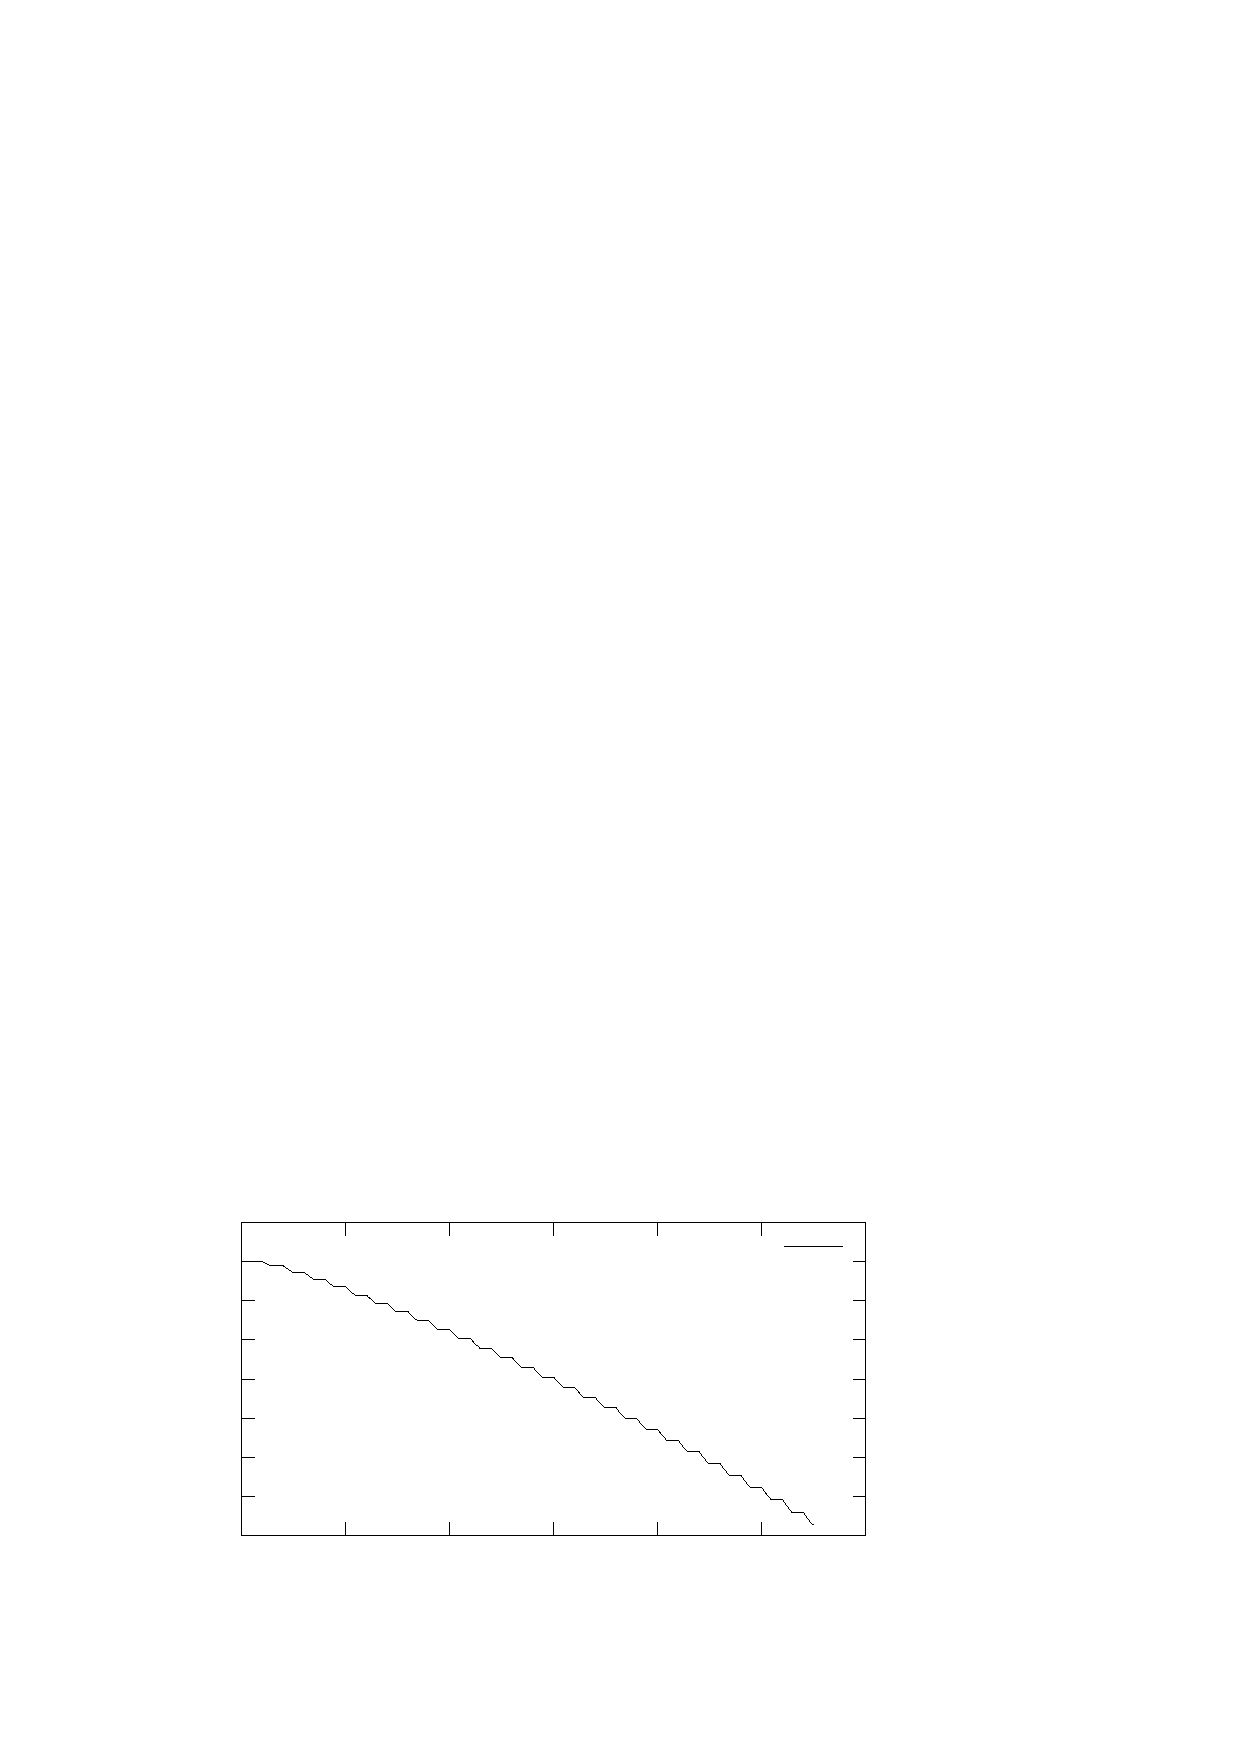
\includegraphics{acefSimpleIntegrator}%
\end{picture}%
\begingroup
\setlength{\unitlength}{0.0200bp}%
\begin{picture}(18000,10800)(0,0)%
\put(1925,1650){\makebox(0,0)[r]{\strut{}-70}}%
\put(1925,2588){\makebox(0,0)[r]{\strut{}-60}}%
\put(1925,3525){\makebox(0,0)[r]{\strut{}-50}}%
\put(1925,4463){\makebox(0,0)[r]{\strut{}-40}}%
\put(1925,5400){\makebox(0,0)[r]{\strut{}-30}}%
\put(1925,6338){\makebox(0,0)[r]{\strut{}-20}}%
\put(1925,7275){\makebox(0,0)[r]{\strut{}-10}}%
\put(1925,8213){\makebox(0,0)[r]{\strut{} 0}}%
\put(1925,9150){\makebox(0,0)[r]{\strut{} 10}}%
\put(2200,1100){\makebox(0,0){\strut{} 0}}%
\put(4696,1100){\makebox(0,0){\strut{} 1e-06}}%
\put(7192,1100){\makebox(0,0){\strut{} 2e-06}}%
\put(9688,1100){\makebox(0,0){\strut{} 3e-06}}%
\put(12183,1100){\makebox(0,0){\strut{} 4e-06}}%
\put(14679,1100){\makebox(0,0){\strut{} 5e-06}}%
\put(17175,1100){\makebox(0,0){\strut{} 6e-06}}%
\put(550,5400){\rotatebox{90}{\makebox(0,0){\strut{}U45}}}%
\put(9687,275){\makebox(0,0){\strut{}time}}%
\put(9687,9975){\makebox(0,0){\strut{}Output U45}}%
\put(14950,8575){\makebox(0,0)[r]{\strut{}"Acef Simple integrator"}}%
\end{picture}%
\endgroup
\endinput


\subsection{ Integrator with a comparator}
It consists in adding a comparator between the output and the input of the integrator. Consequently,
the output signal will oscillate between a positive and a negative value. So, the operating point of
the circuit will go through the non regularity of the comparator, and may be will cause some problems of
convergence.

\begin{figure}[!h]
\centerline{
 \scalebox{0.7}{
    \input{compIntegrator.pstex_t}
 }
 }\end{figure}



\subsubsection{Phase 2}
The equivalent circuit is:

Because the value of the gate $V_{g}=5V$ and $V_{T}=0.5$, the current trough the MOS is given by the following equation:
\[I_{ds}=F(V_{d},V_{s})=K *((V_{gs}-V_{T})*V_{ds} - \frac{1}{2}*V_{ds}^2 \]
The equation of the system is :\\
$V_{1}, V_{4}$ and $V_{6}$ are constants.\\
$(V_{2} - V_{3})$ is continuous because of capacitor $C_{1}$, it is necessary to compute the initial values.
\begin{eqnarray}
F(V_{3},0)=-F(V_{2},V_{1})\\
C_{1}\frac{d(V2-V3)}{dt} = -F(V_{2},V_{1})\\
\end{eqnarray}


\subsubsection{Phase 1}
The equivalent circuit is:

Because the value of the gate $V_{g}=5V$ and $V_{T}=0.5$, the current trough the MOS is given by the following equation:
\[I_{ds}=F(V_{d},V_{s})=K *((V_{gs}-V_{T})*V_{ds} - \frac{1}{2}*V_{ds}^2 \]
The equation of the system is :\\
$(V_{2} - V_{3})$ and  $(V_{4} - V_{5})$ ar continuous because of capacitor $C_{1}$, it is necessary to compute the initial values.
\begin{eqnarray}
F(V_{3},V_{4})=-F(V_{2},0)\\
C_{1}\frac{d(V_{2}-V_{3})}{dt} = -F(V_{2},0)\\
C_{2}\frac{d(V_{4}-V_{5})}{dt} = -F(V_{2},0)\\
V_{5}=\alpha*V_{4}\\
V_{1}=comp(V_{4}-V_{5})\\
\end{eqnarray}

\subsubsection{Acef simulation}
The Maple integration of these previous systems validates the ACEF simulation. Many simulations have
been perform by changed some parameters values.

%GNUPLOT: LaTeX picture with Postscript
\begin{picture}(0,0)%
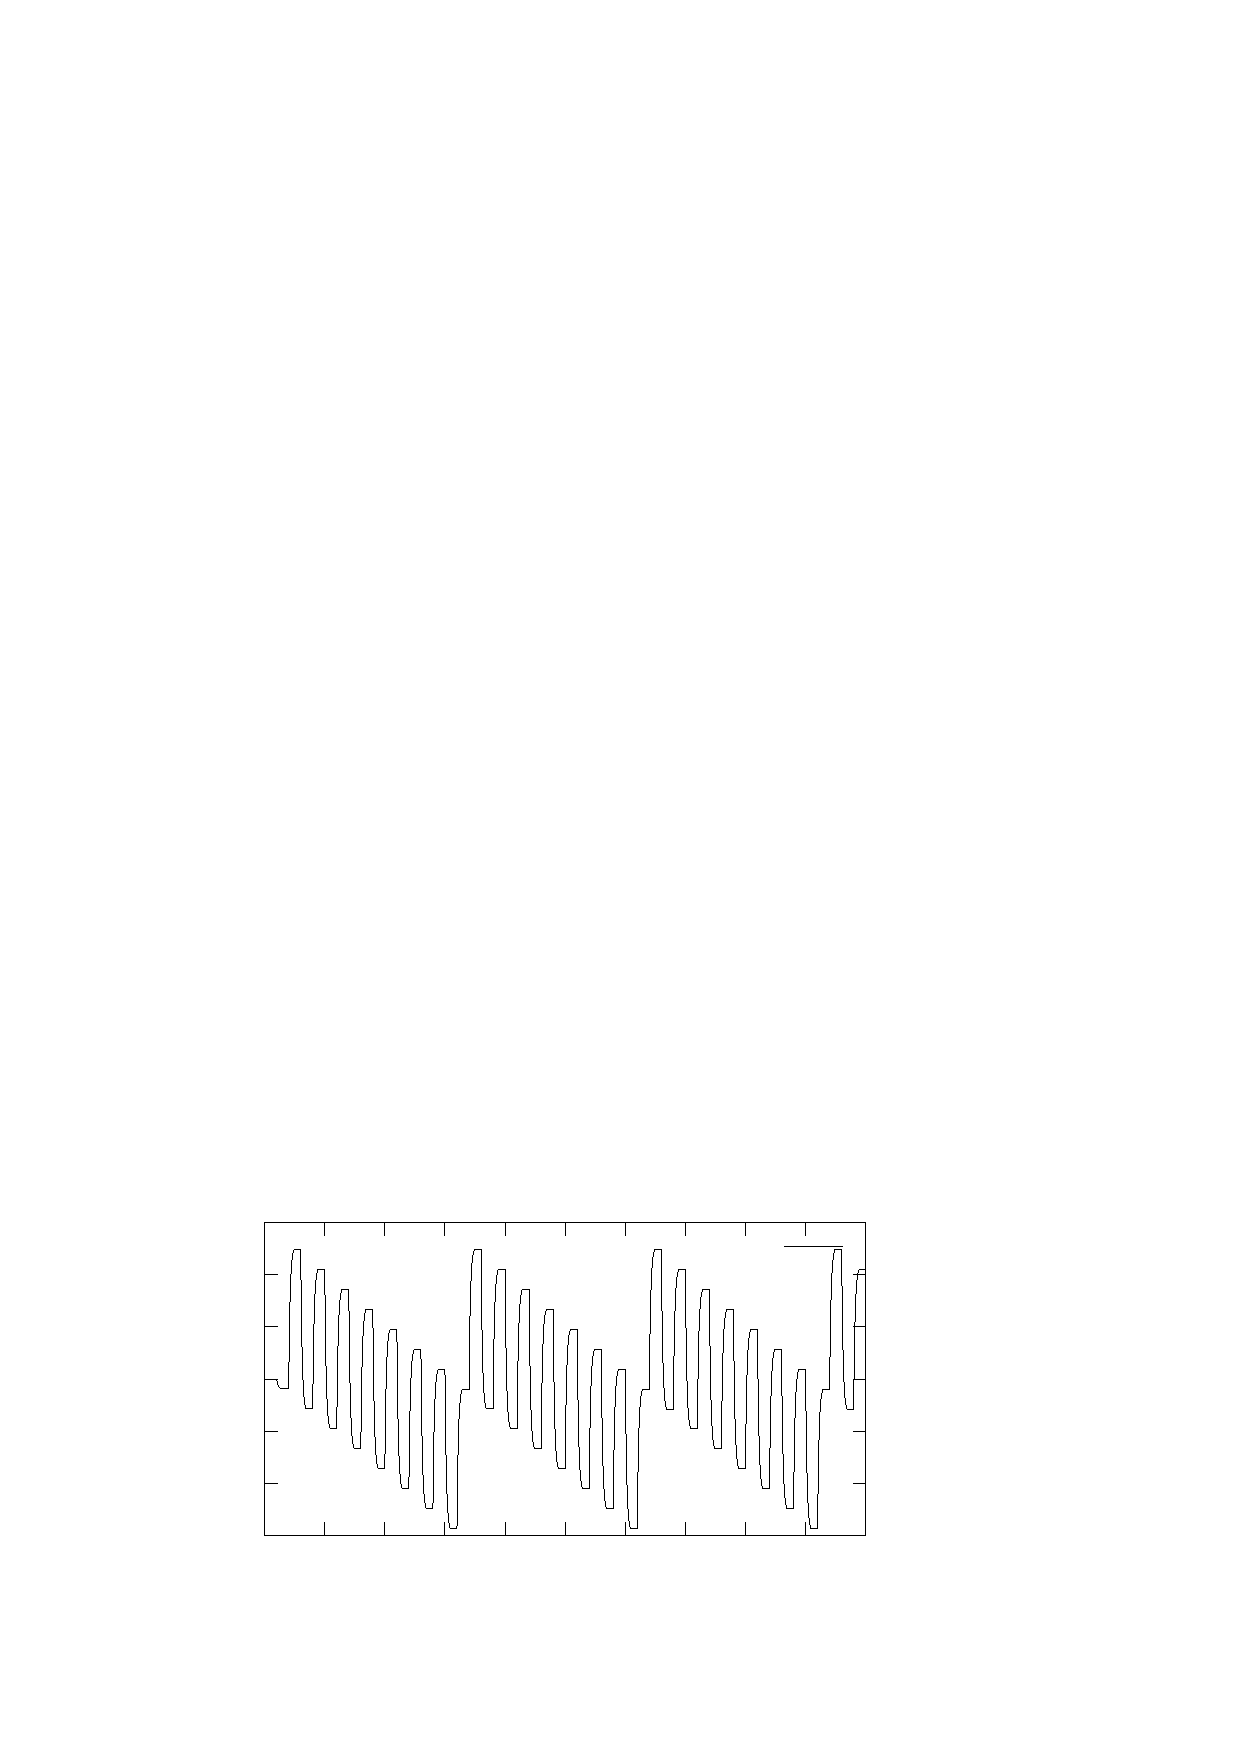
\includegraphics{acefCompIntegrator}%
\end{picture}%
\begingroup
\setlength{\unitlength}{0.0200bp}%
\begin{picture}(18000,10800)(0,0)%
\put(2475,1650){\makebox(0,0)[r]{\strut{}-0.15}}%
\put(2475,2900){\makebox(0,0)[r]{\strut{}-0.1}}%
\put(2475,4150){\makebox(0,0)[r]{\strut{}-0.05}}%
\put(2475,5400){\makebox(0,0)[r]{\strut{} 0}}%
\put(2475,6650){\makebox(0,0)[r]{\strut{} 0.05}}%
\put(2475,7900){\makebox(0,0)[r]{\strut{} 0.1}}%
\put(2475,9150){\makebox(0,0)[r]{\strut{} 0.15}}%
\put(2750,1100){\makebox(0,0){\strut{} 0}}%
\put(4193,1100){\makebox(0,0){\strut{} 1e-06}}%
\put(5635,1100){\makebox(0,0){\strut{} 2e-06}}%
\put(7078,1100){\makebox(0,0){\strut{} 3e-06}}%
\put(8520,1100){\makebox(0,0){\strut{} 4e-06}}%
\put(9963,1100){\makebox(0,0){\strut{} 5e-06}}%
\put(11405,1100){\makebox(0,0){\strut{} 6e-06}}%
\put(12848,1100){\makebox(0,0){\strut{} 7e-06}}%
\put(14290,1100){\makebox(0,0){\strut{} 8e-06}}%
\put(15733,1100){\makebox(0,0){\strut{} 9e-06}}%
\put(17175,1100){\makebox(0,0){\strut{} 1e-05}}%
\put(550,5400){\rotatebox{90}{\makebox(0,0){\strut{}U45}}}%
\put(9962,275){\makebox(0,0){\strut{}time}}%
\put(9962,9975){\makebox(0,0){\strut{}acef Comparator-Integrator}}%
\put(14950,8575){\makebox(0,0)[r]{\strut{}"Acef Comparator Integrator"}}%
\end{picture}%
\endgroup
\endinput


\subsubsection{Simulation with ELDO}
During the simulation, it appears a lot of messages about a non convergence of the Newton method.
Moreover it is possible to get a large panel of simulation by changed the comparator coefficient.\\

\begin{figure}[!h]
comparator : Ecomp 1 0 VALUE={0.1 -1.5*tanh(100*(V(5)-V(4)))}
\begin{center}
 \scalebox{0.1}{
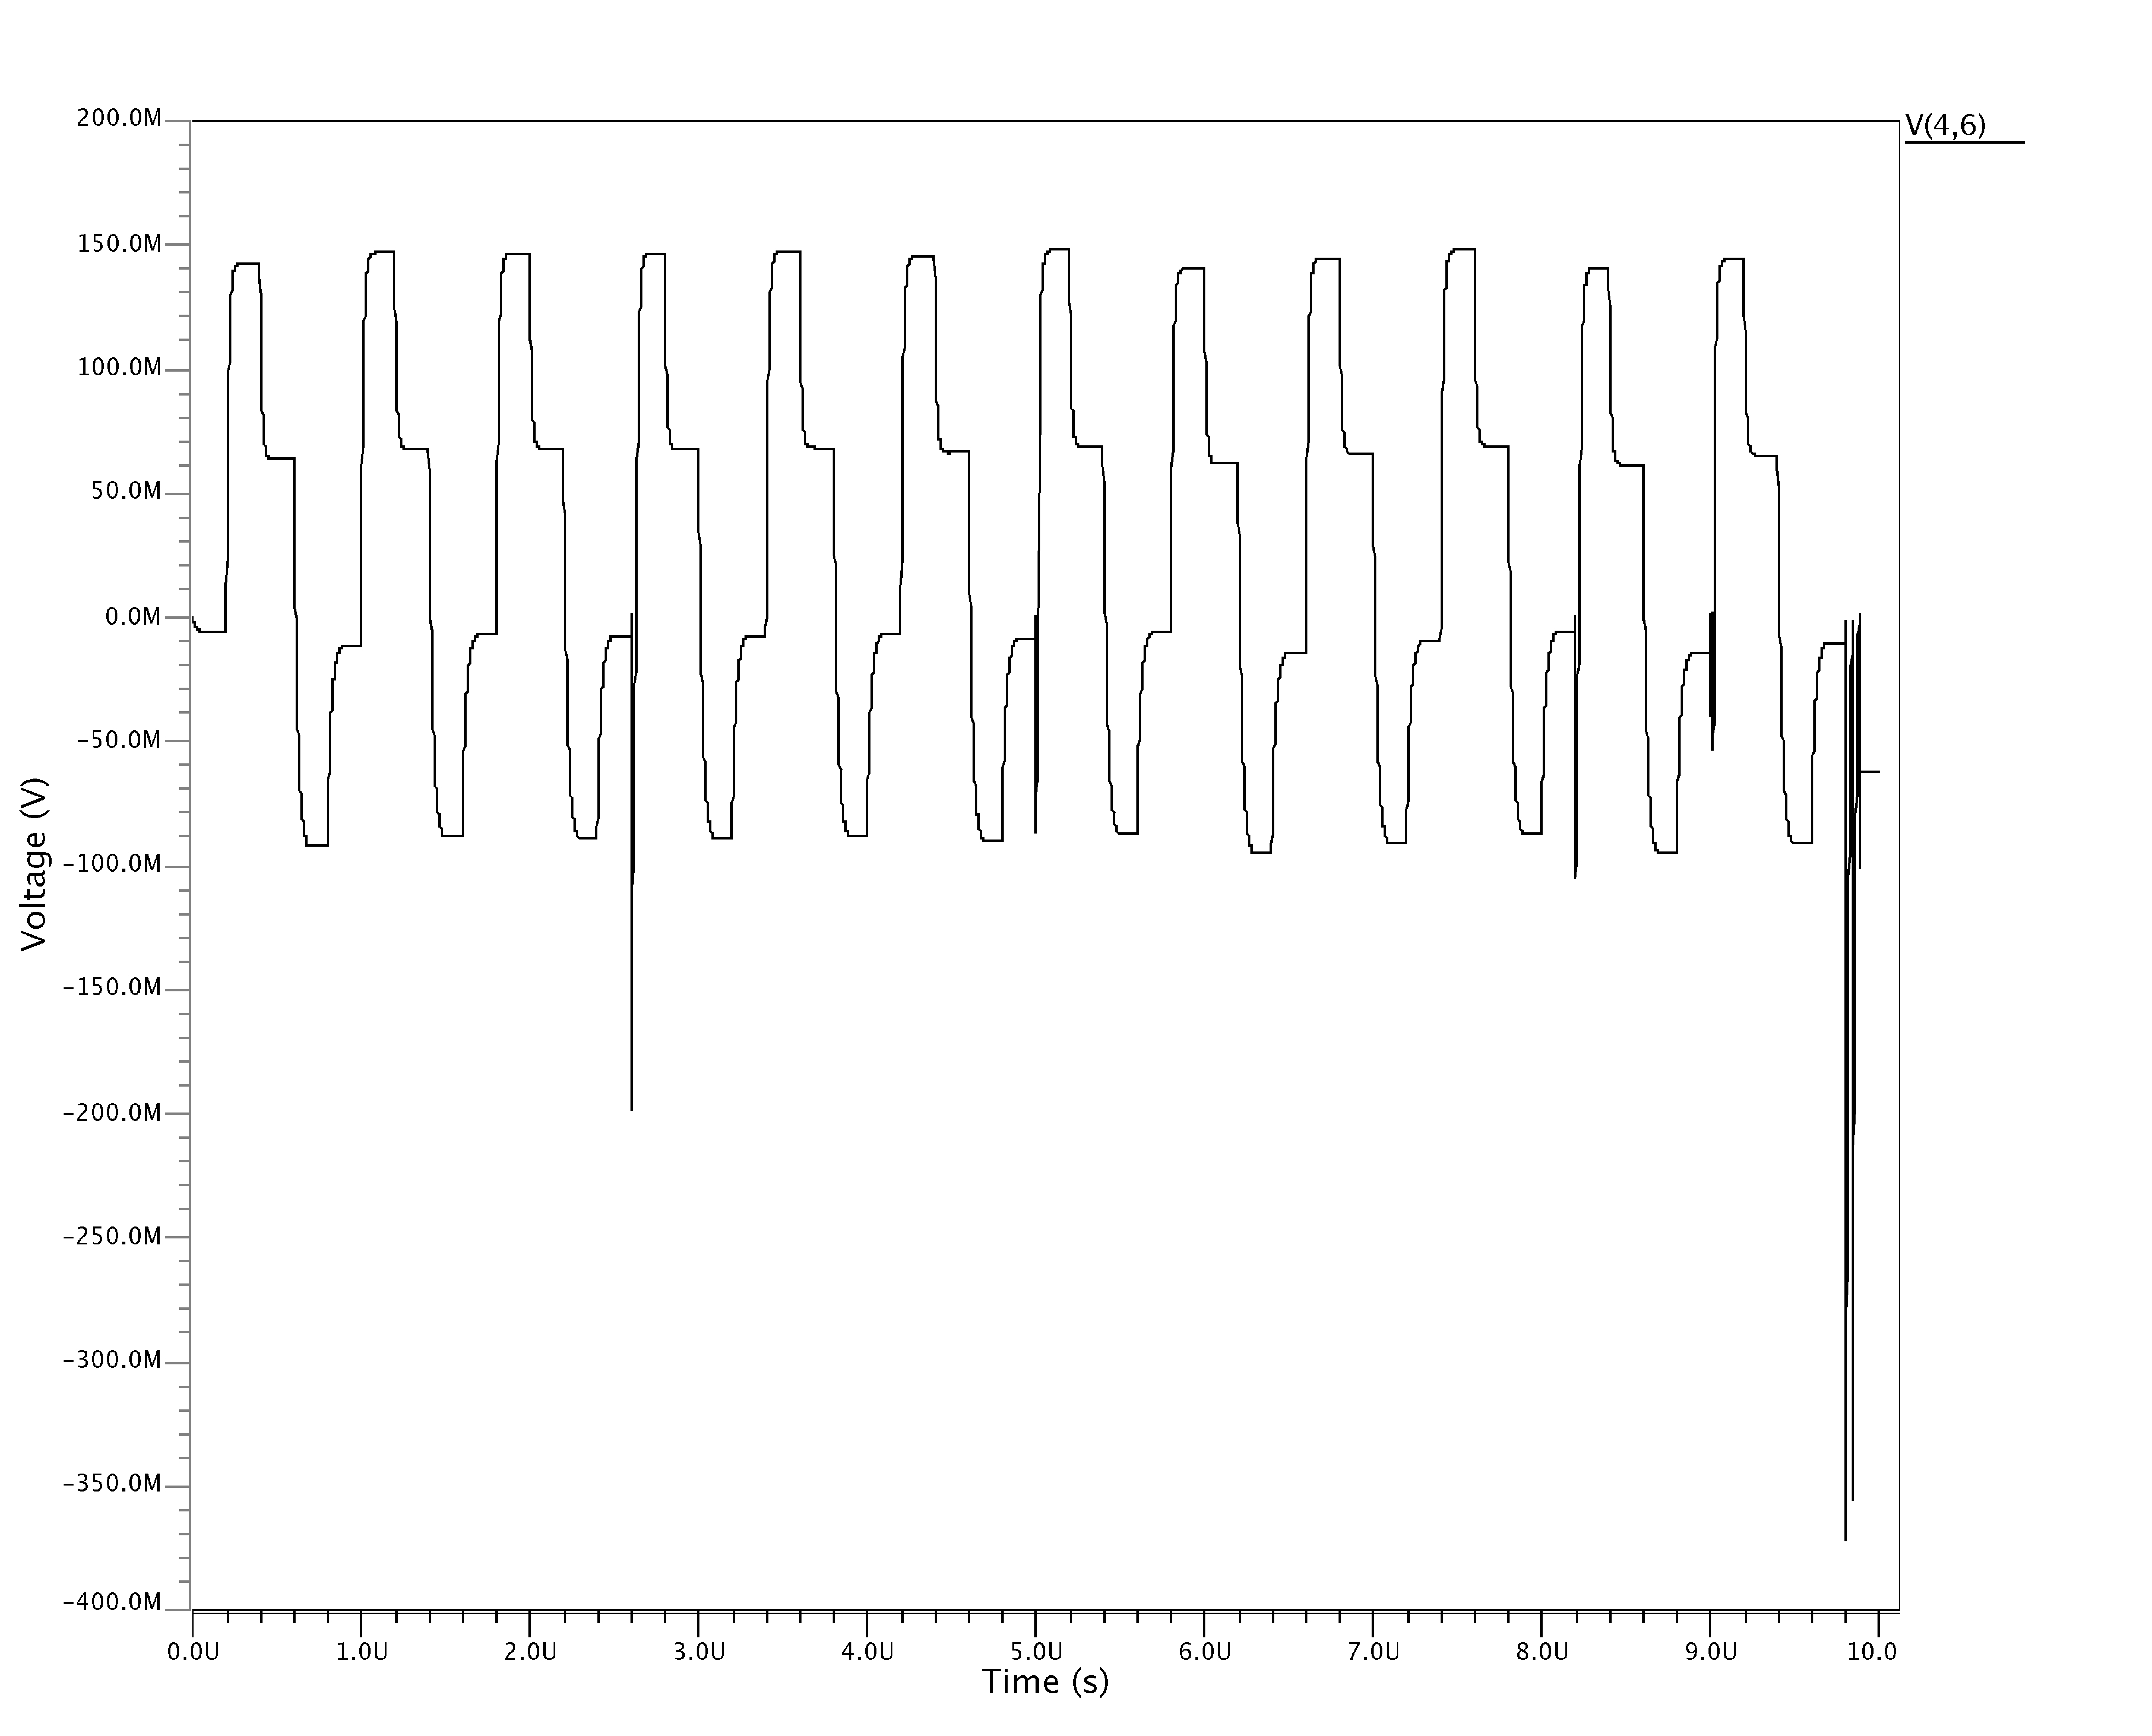
\includegraphics{EldoCompInt100.eps}
}
\end{center}

\end{figure}
\begin{figure}[!h]
comparator : Ecomp 1 0 VALUE={0.1 -1.5*tanh(1000*(V(5)-V(4)))}
\begin{center}
 \scalebox{0.1}{
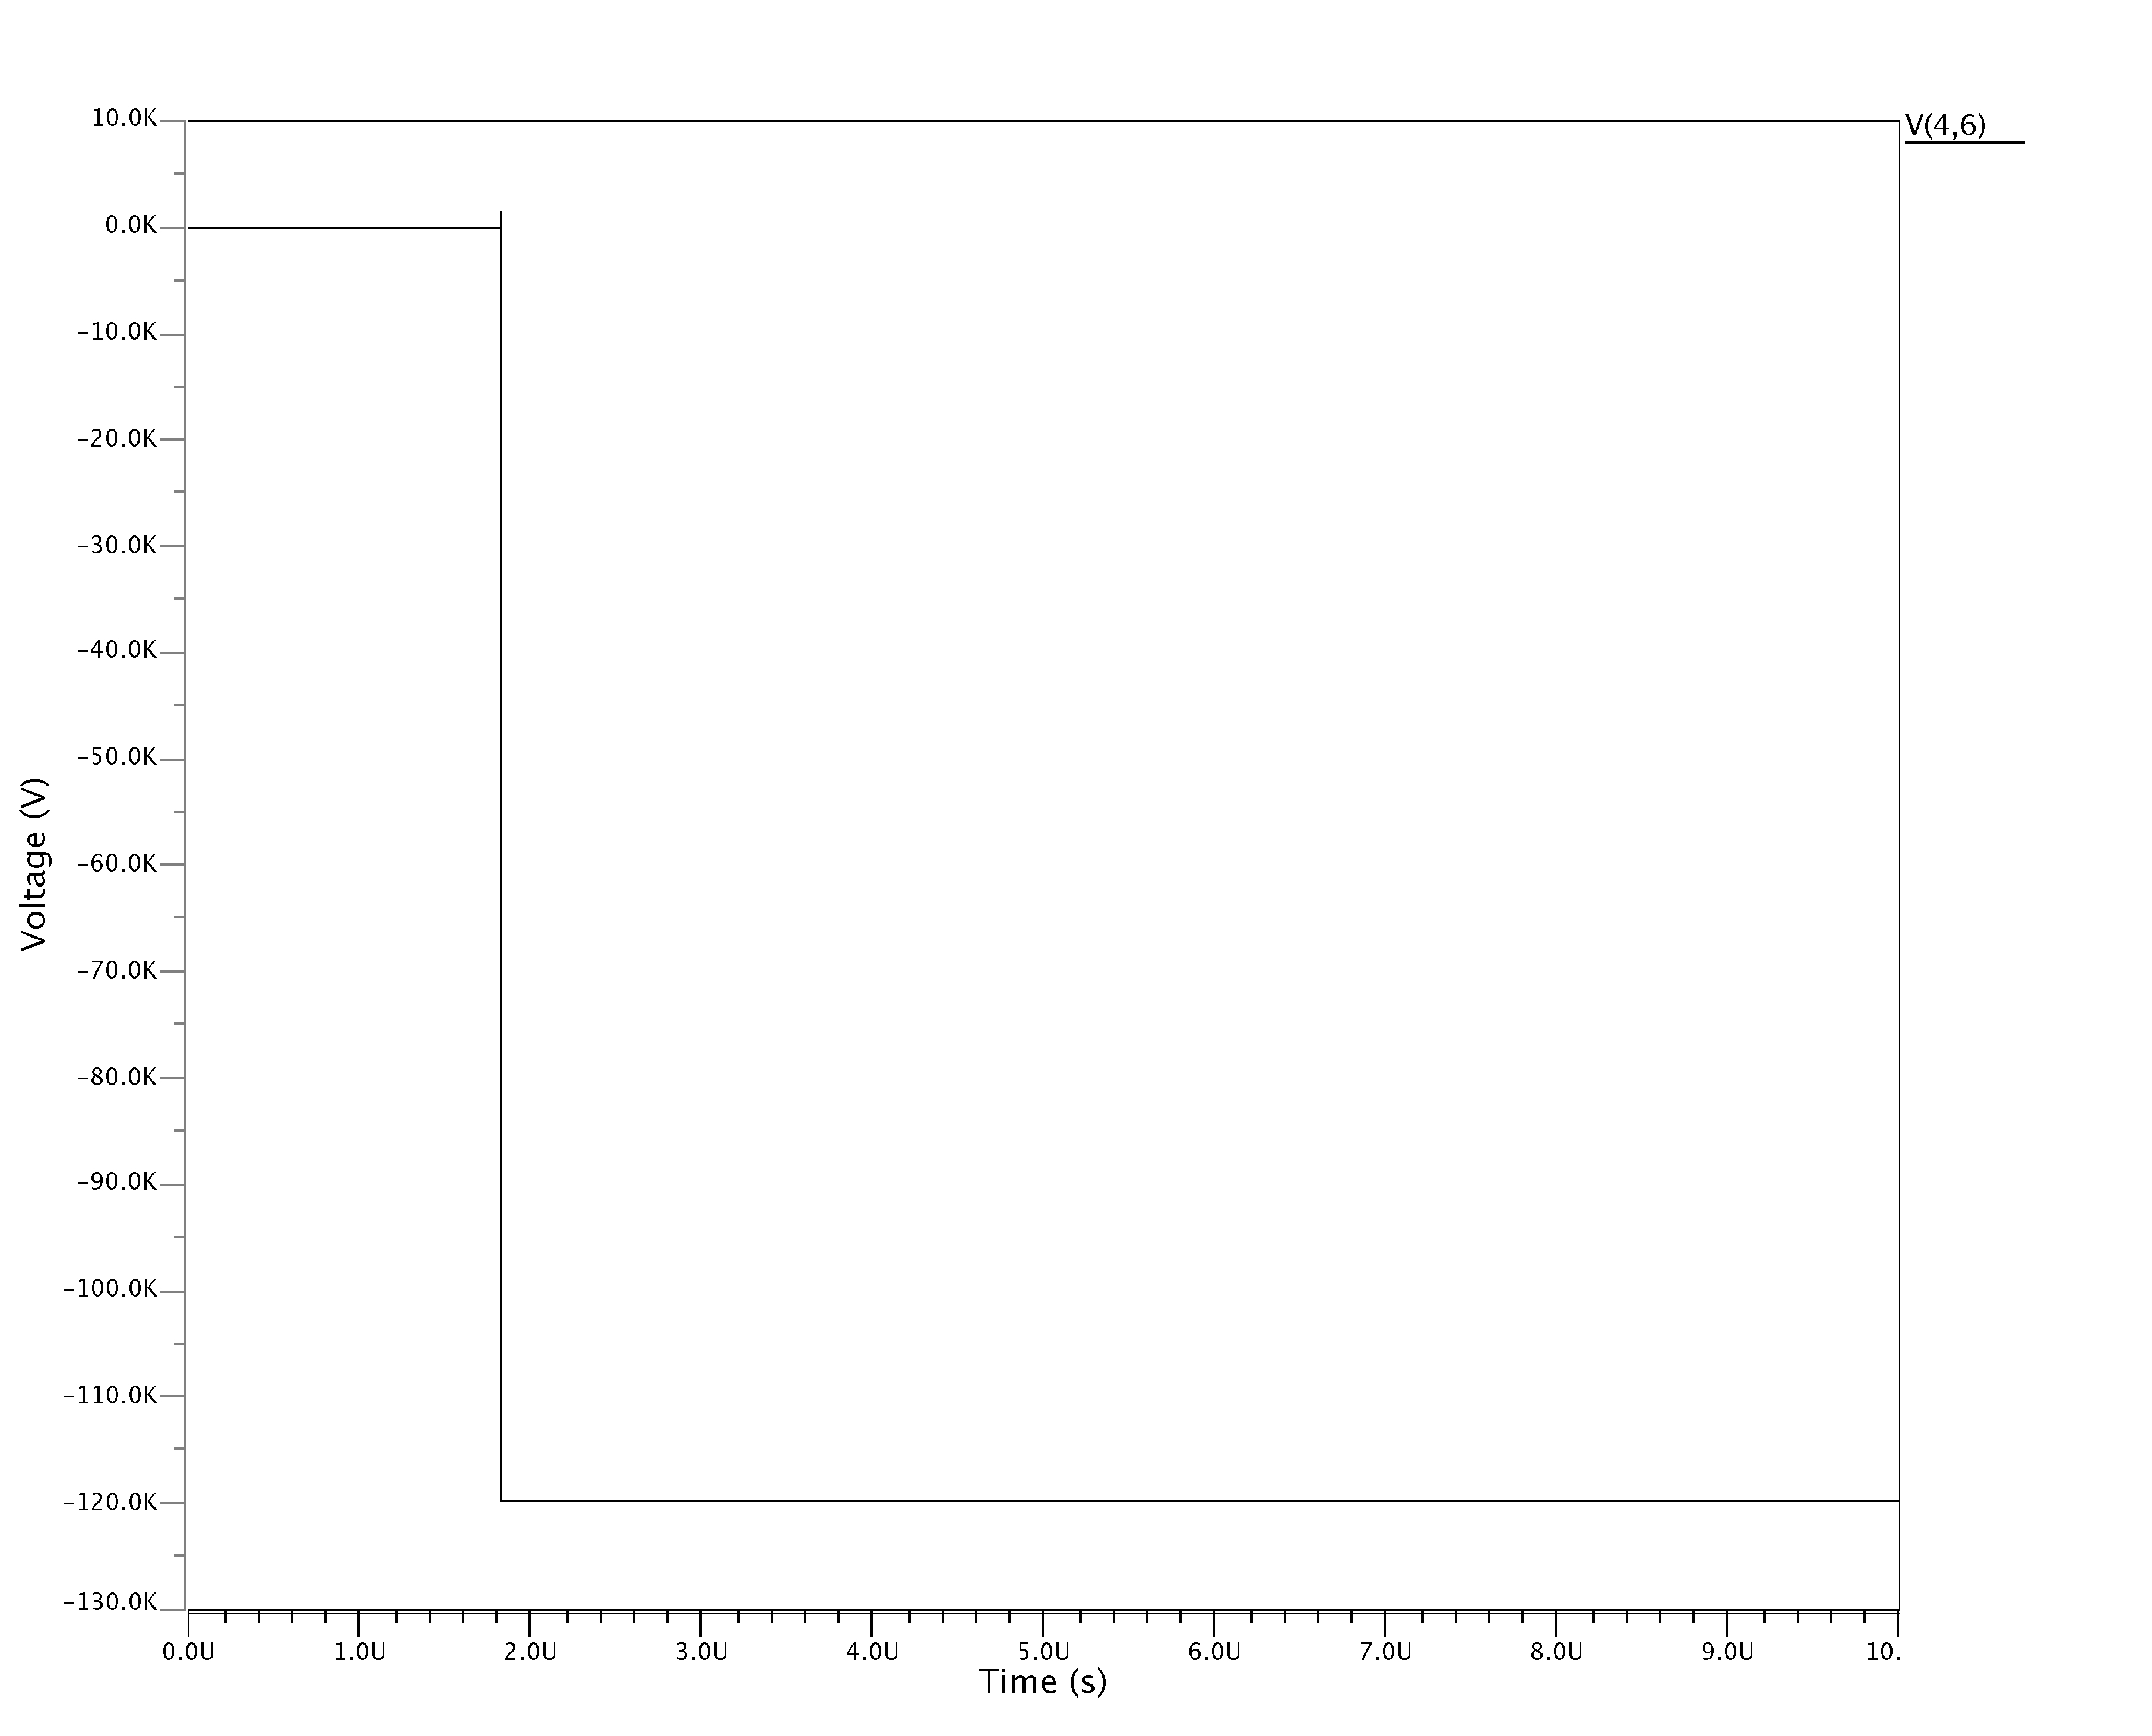
\includegraphics{EldoCompInt1000.eps}
}
\end{center}
\end{figure}
\begin{figure}[!h]
comparator : Ecomp 1 0 VALUE={0.1 -1.5*tanh(10000*(V(5)-V(4)))}
\begin{center}
 \scalebox{0.1}{
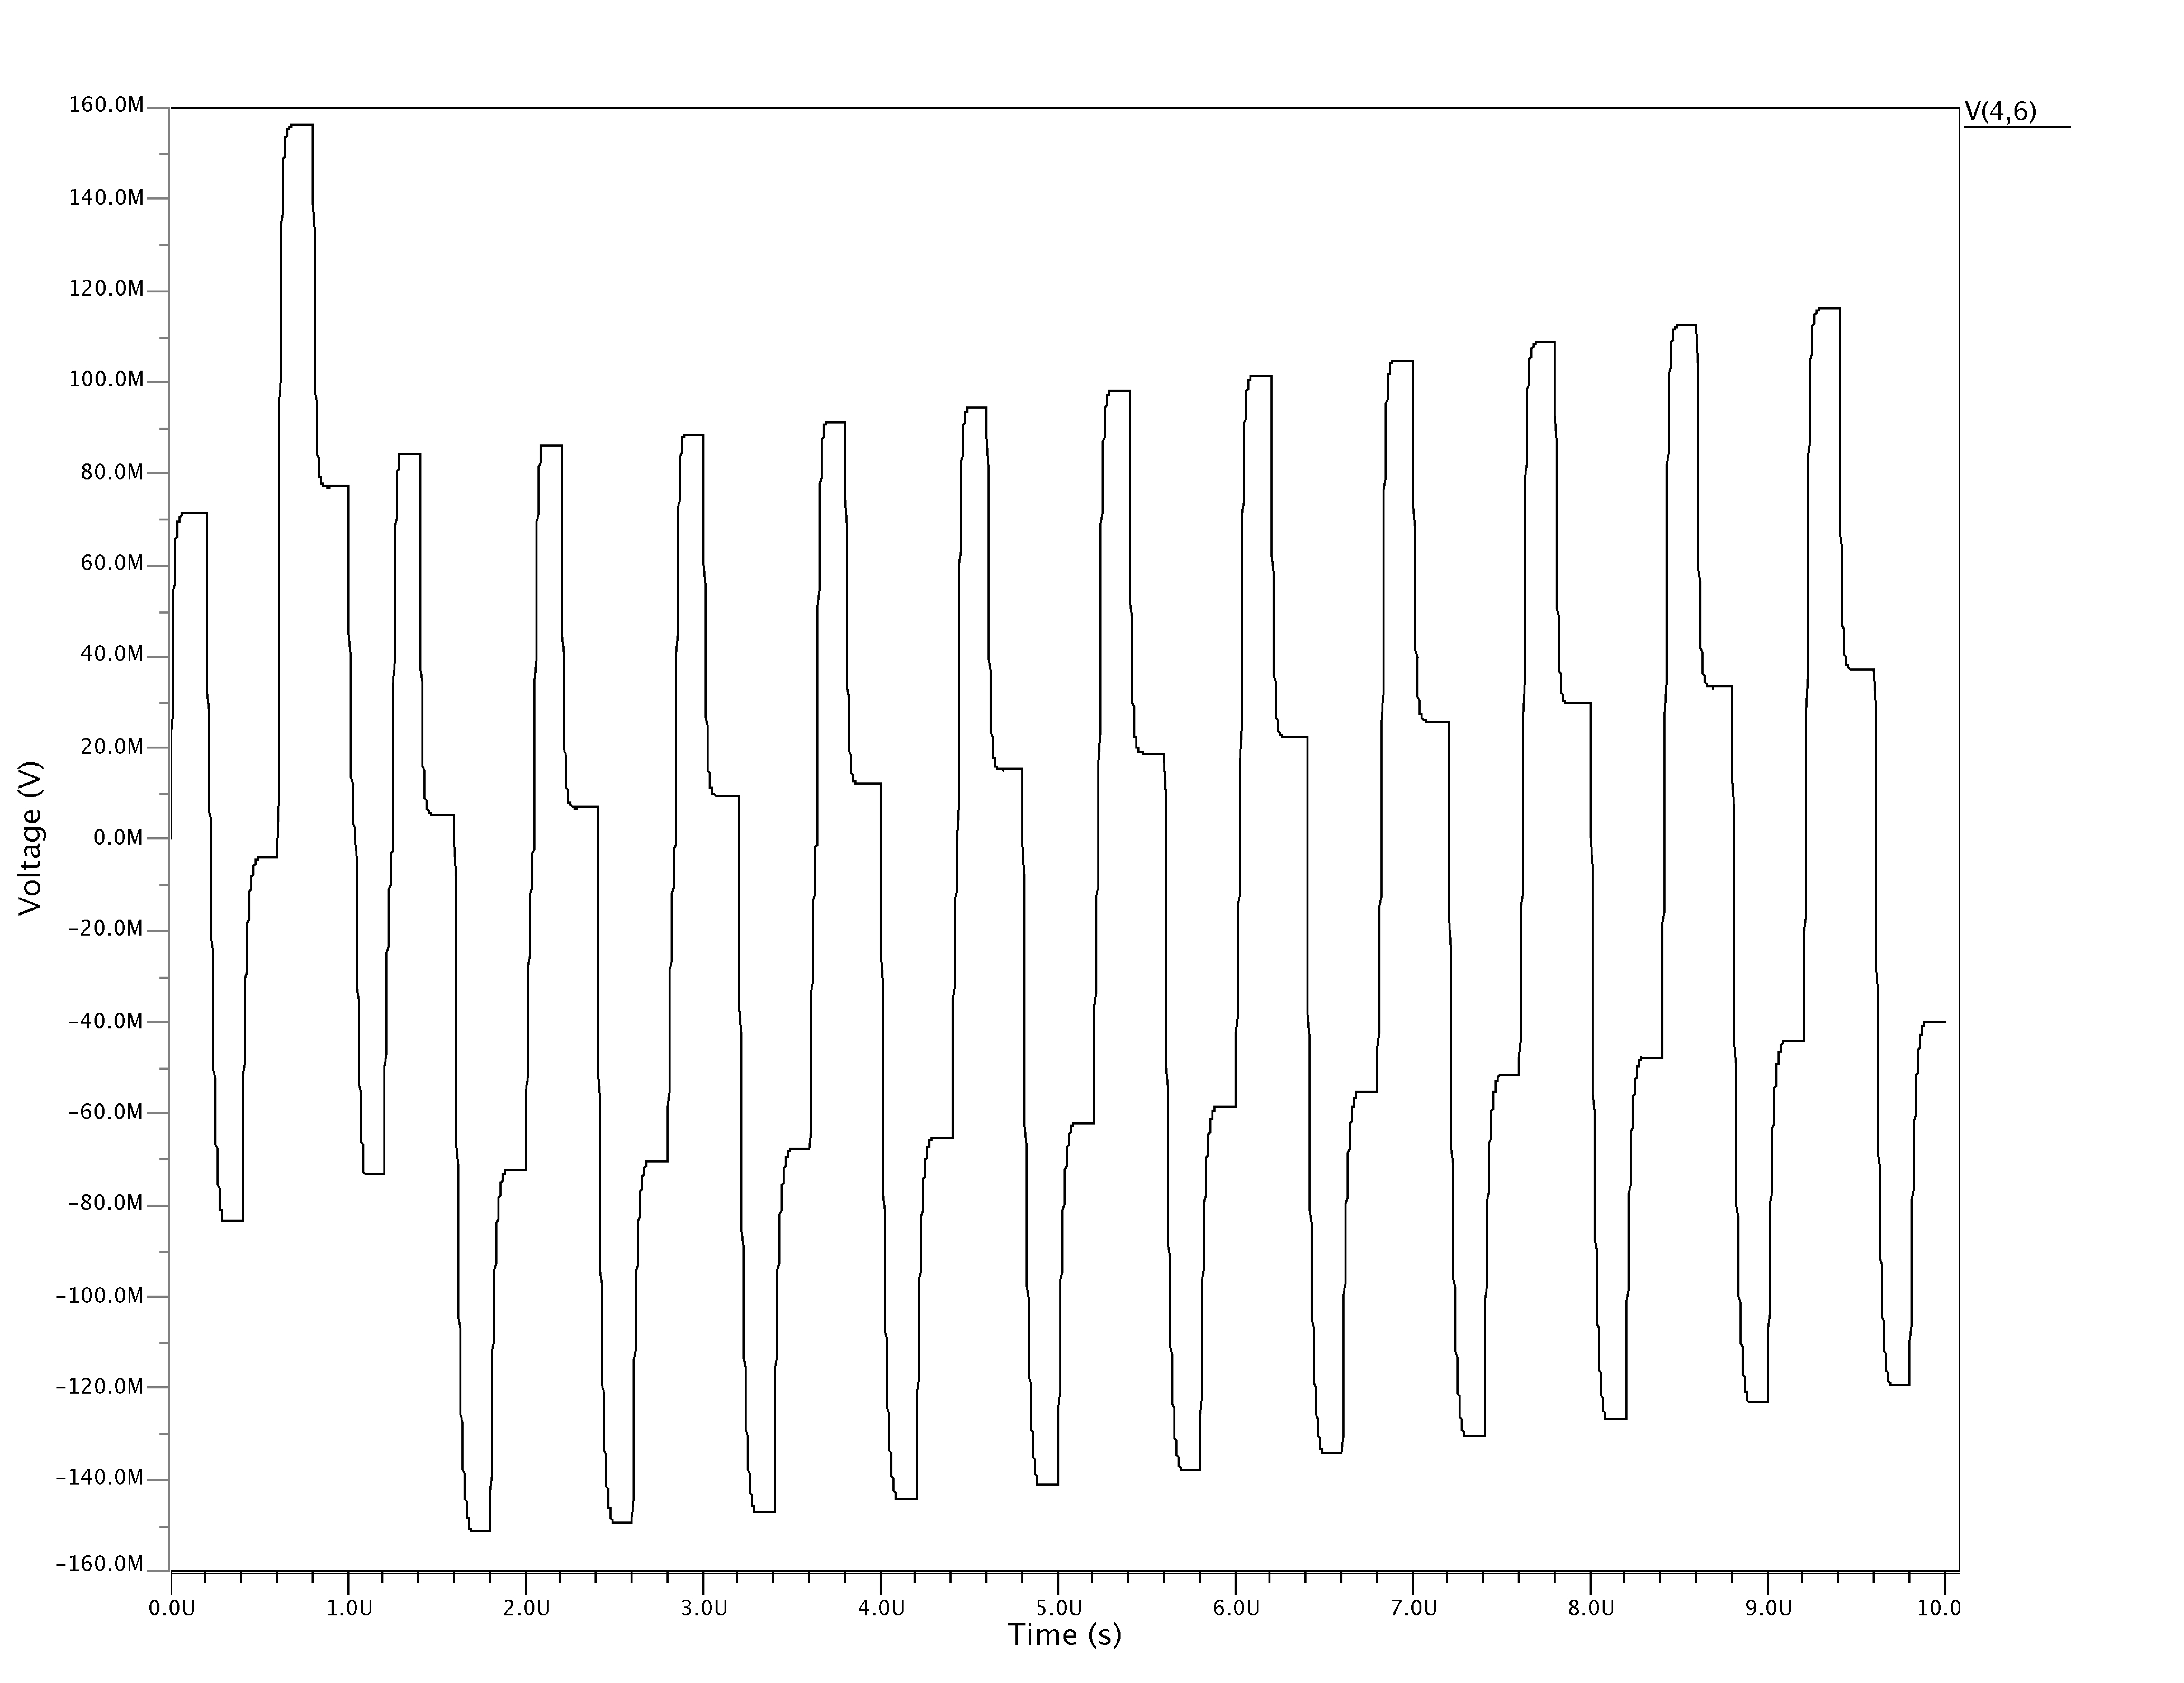
\includegraphics{EldoCompInt10000.eps}
}
\end{center}
\end{figure}
\begin{figure}[!h]
A new set of value for $C_{1}$ and $C_{2}$
\begin{center}
 \scalebox{0.1}{
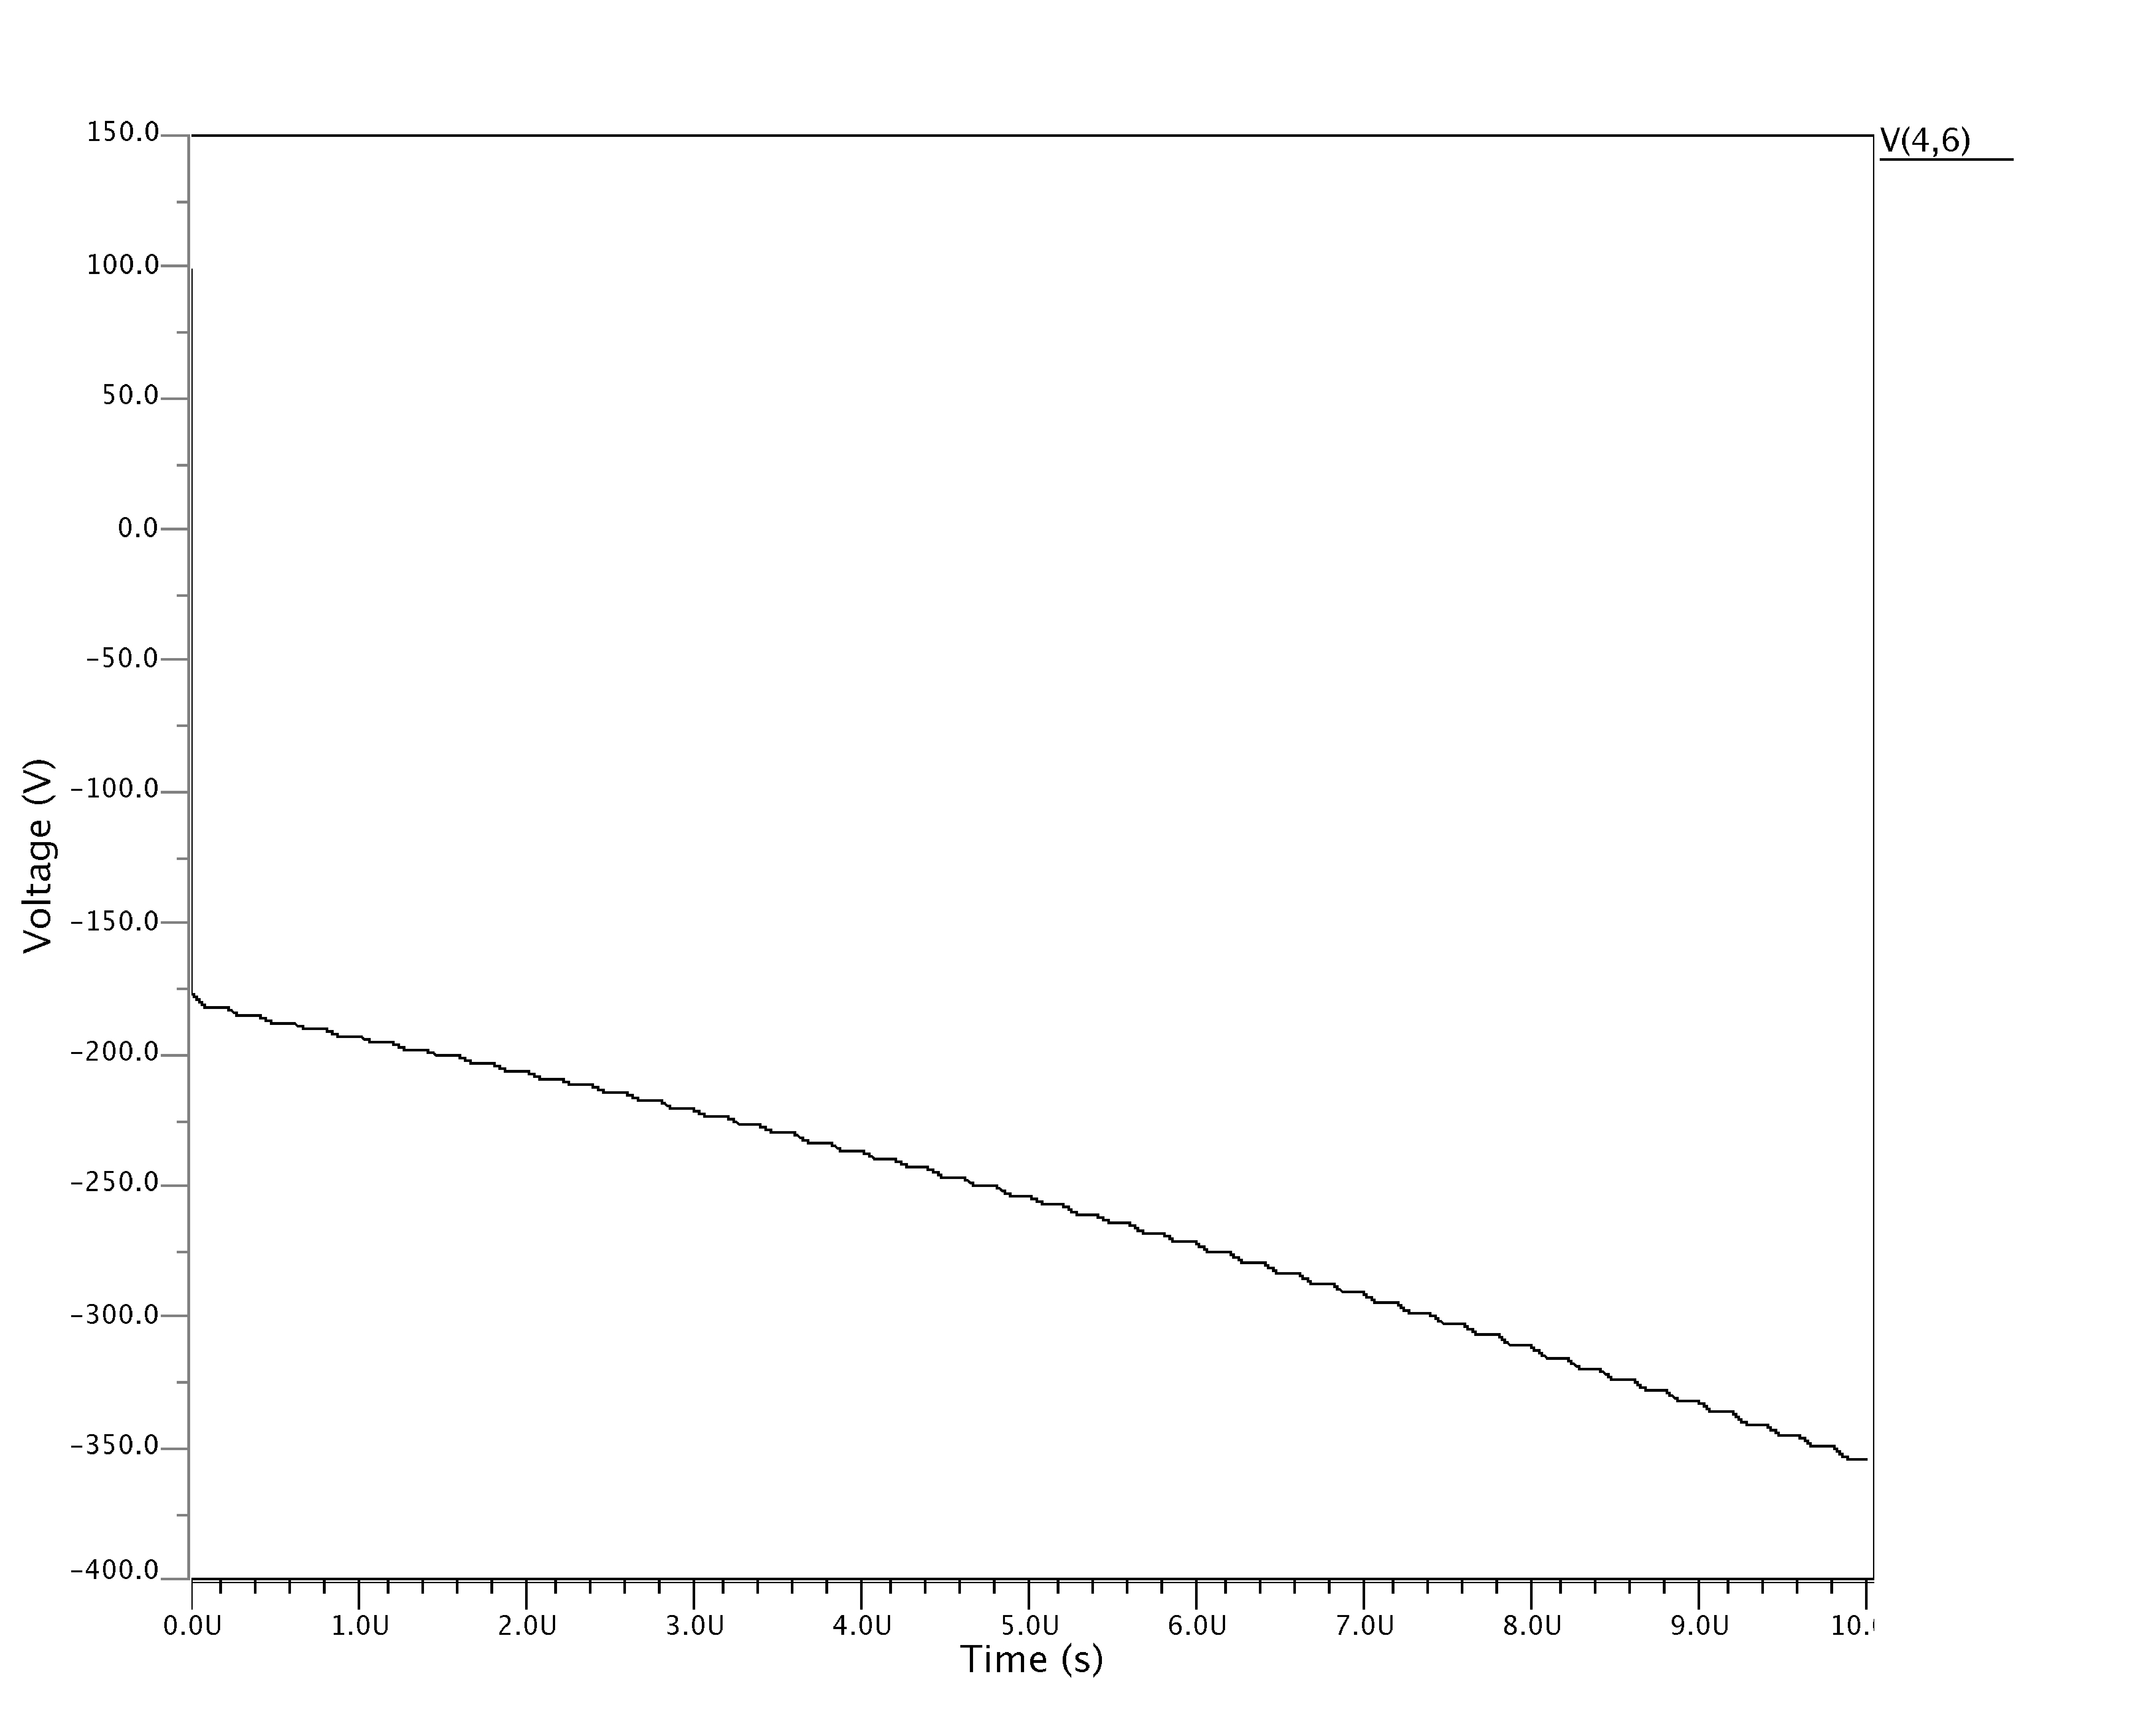
\includegraphics{EldoCompIntCap.eps}
}
\end{center}
\end{figure}

\newpage
